\documentclass[a4paper,11pt]{article}

\usepackage[dutch]{babel}
\usepackage[utf8]{inputenc}
\usepackage{amsmath}
\usepackage{amssymb}
\usepackage{geometry}
\usepackage{enumitem}
\usepackage{graphicx}
\usepackage{tikz}
\usepackage[hidelinks]{hyperref}

\geometry{margin=2.5cm}

\title{Oefeningen Wiskunde voor Systemen}
\author{KU Leuven - ESAT}
\date{\today}

\begin{document}

\maketitle
\tableofcontents
\newpage

\section{Formularium}
\label{sec:formularium}

Dit formularium is een compacte samenvatting van de standaardformules uit het ``Signals and Systems'' formularium. In de oefeningen wordt hiernaar verwezen.

\subsection{Laplace transform (LT)}
\label{form:laplace}

\subsubsection*{1.1 Definitie en eigenschappen}
\label{form:laplace-def}
\label{form:laplace-prop}
\begingroup
\setlength{\tabcolsep}{6pt}
\renewcommand{\arraystretch}{1.35}
\[
\begin{array}{@{}lcl@{}}
\text{Definitie:} & f(t)\,u(t) & \longleftrightarrow\; F(s)=\displaystyle\int_0^{\infty} f(t)e^{-st}\,dt\\
\text{translatie in } s: & f(t)e^{-at}\,u(t) & \longleftrightarrow\; F(s+a)\\
\text{translatie in } t: & f(t-a)\,u(t-a) & \longleftrightarrow\; e^{-as}F(s)\\
\text{afgeleide in } t: & \dfrac{d}{dt}\big(f(t)u(t)\big) & \longleftrightarrow\; sF(s)-f(0^+)\\
 & \dfrac{d^2}{dt^2}\big(f(t)u(t)\big) & \longleftrightarrow\; s^2F(s)-s f(0^+)-f'(0^+)\\

\text{afgeleide in } s: & t\,f(t)\,u(t) & \longleftrightarrow\; -\dfrac{d}{ds}F(s)\\
 & t^n f(t)\,u(t) & \longleftrightarrow\; (-1)^n\,\dfrac{d^n}{ds^n}F(s)\\
\text{convolutie:} & \big(f*g\big)(t)\,u(t) & \longleftrightarrow\; F(s)\,G(s)\\
\text{schaling:} & f(a t) & \longleftrightarrow\; \dfrac{1}{a}\,F\!\left(\dfrac{s}{a}\right)\\
\end{array}
\]
\endgroup

\noindent\textbf{Initial value theorem:}
\[
\lim_{t\to 0^+} f(t)=\lim_{s\to\infty} sF(s).
\]
\noindent\textbf{Final value theorem:}
\[
\lim_{t\to\infty} f(t)=\lim_{s\to 0} sF(s)\quad(\text{onder de gebruikelijke poolvoorwaarden}).
\]
\noindent\textbf{Link met FTC:}
\label{form:lt-ft-link}
\[
\mathrm{LT}(s=j\omega)=\mathrm{FTC}(j\omega)\quad \text{als } x(t) \text{ absoluut integreerbaar is.}
\]

\subsubsection*{1.2 Useful Laplace pairs}
\label{form:laplace-pairs}
\begingroup
\setlength{\tabcolsep}{10pt}
\renewcommand{\arraystretch}{1.35}
\[
\begin{array}{@{}lcl@{\qquad}lcl@{}}
e^{-at}u(t) & \longleftrightarrow & \dfrac{1}{s+a} & t^n u(t) & \longleftrightarrow & \dfrac{n!}{s^{n+1}}\\
\cos(a t)u(t) & \longleftrightarrow & \dfrac{s}{s^2+a^2} & \sin(a t)u(t) & \longleftrightarrow & \dfrac{a}{s^2+a^2}\\
\delta(t) & \longleftrightarrow & 1 & u(t) & \longleftrightarrow & \dfrac{1}{s}\\
t\cos(a t)u(t) & \longleftrightarrow & \dfrac{s^2-a^2}{(s^2+a^2)^2} & t\sin(a t)u(t) & \longleftrightarrow & \dfrac{2sa}{(s^2+a^2)^2}
\end{array}
\]
\endgroup

\subsection{Fourier transform (FTC)}
\label{form:ft}

\subsubsection*{2.1 Basic formulae}
\label{form:ft-def}
\label{form:ft-prop}
\[
X(\omega)=\int_{-\infty}^{\infty} x(t)e^{-j\omega t}\,dt,\qquad
x(t)=\frac{1}{2\pi}\int_{-\infty}^{\infty} X(\omega)e^{j\omega t}\,d\omega.
\]

\begingroup
\setlength{\tabcolsep}{6pt}
\renewcommand{\arraystretch}{1.35}
\[
\begin{array}{@{}lcl@{}}
\text{convolution theorem (tijd):} & f(t)*g(t) & \longleftrightarrow\; F(\omega)\,G(\omega)\\
\text{convolution theorem (freq.):} & f(t)\,g(t) & \longleftrightarrow\; \dfrac{1}{2\pi}\,(F*G)(\omega)\\
\text{translatie:} & x(t-t_0) & \longleftrightarrow\; X(\omega)e^{-j\omega t_0}\\
\text{symmetry (reëel $x$):} &  & X(-\omega)=X^*(\omega)\\
\text{time symmetry (reëel $x$):} & x(-t) & \longleftrightarrow\; X(-\omega)=X^*(\omega)\\
\text{link FS--FTC:} &  & X(k\omega_0)=T\,c_k\quad(\omega_0=2\pi/T)
\end{array}
\]
\endgroup

\subsubsection*{2.2 Useful Fourier pairs}
\label{form:ft-pairs}
We gebruiken $\mathrm{sinc}(x)=\dfrac{\sin(x)}{x}$.

\begingroup
\setlength{\tabcolsep}{8pt}
\renewcommand{\arraystretch}{1.4}
\[
\begin{array}{@{}lcl@{}}
\text{Block:} & x(t)=\begin{cases}A,& t\in[-L/2,L/2]\\0,& \text{elders}\end{cases}
& \longleftrightarrow\; X(\omega)=AL\,\mathrm{sinc}\!\left(\dfrac{\omega L}{2}\right)\\
\text{Sinc:} & x(t)=A\,\mathrm{sinc}(\omega_0 t)
& \longleftrightarrow\; X(\omega)=\begin{cases}\dfrac{A\pi}{\omega_0},& |\omega|<\omega_0\\0,& \text{elders}\end{cases}\\
\text{Impuls:} & \delta(t-t_0) & \longleftrightarrow\; e^{-j\omega t_0}\\
\text{Complex expon.:} & e^{j\omega_0 t} & \longleftrightarrow\; 2\pi\,\delta(\omega-\omega_0)\\
\text{Cosine:} & \cos(\omega_0 t) & \longleftrightarrow\; \pi\,[\delta(\omega+\omega_0)+\delta(\omega-\omega_0)]\\
\text{Sine:} & \sin(\omega_0 t) & \longleftrightarrow\; j\pi\,[\delta(\omega+\omega_0)-\delta(\omega-\omega_0)]\\
\text{Delta train:} & \sum\limits_{k=-\infty}^{\infty}\delta(t-kT) & \longleftrightarrow\; \dfrac{2\pi}{T}\sum\limits_{k=-\infty}^{\infty}\delta\!\left(\omega-\dfrac{2\pi k}{T}\right)
\end{array}
\]
\endgroup

\subsection{Fourier series (FS)}
\label{form:fs}

\subsubsection*{3.1 Cartesian form}
\label{form:fs-cart}
Voor periode $T$ met $\omega_0=\dfrac{2\pi}{T}$:
\[
f(t)=\frac{a_0}{2}+\sum_{k=1}^{\infty}\left[a_k\cos\left(\frac{2\pi k}{T}t\right)+b_k\sin\left(\frac{2\pi k}{T}t\right)\right].
\]
\[
a_0=\frac{2}{T}\int_{0}^{T} f(t)\,dt,\qquad
a_k=\frac{2}{T}\int_{0}^{T} f(t)\cos\left(\frac{2\pi k}{T}t\right)\,dt,\qquad
b_k=\frac{2}{T}\int_{0}^{T} f(t)\sin\left(\frac{2\pi k}{T}t\right)\,dt.
\]

\subsubsection*{3.2 Complex form}
\label{form:fs-cplx}
\[
x(t)=\sum_{k=-\infty}^{\infty} c_k e^{jk\omega_0 t},\qquad \omega_0=\frac{2\pi}{T},\qquad
c_k=\frac{1}{T}\int_{0}^{T} f(t)\,e^{-jk\omega_0 t}\,dt.
\]
\noindent\textbf{symmetry (reëel $f$):}\; $c_{-k}=c_k^*$.

\noindent\textbf{Spectrum:}
\[
X(\omega)=\frac{2\pi}{T}\sum_{k=-\infty}^{\infty} c_k\,\delta(\omega-k\omega_0).
\]

\subsubsection*{3.3 Links between cartesian and complex form}
\label{form:fs-ft-link}
\[
c_k=\frac{a_k-jb_k}{2},\qquad c_k^*=\frac{a_k+jb_k}{2}.
\]
\[
|c_k|=\frac{1}{2}\sqrt{a_k^2+b_k^2},\qquad \varphi_k=\mathrm{Arctan2}(a_k,-b_k).
\]
\[
a_k=2\,\mathrm{Re}\{c_k\},\qquad b_k=-2\,\mathrm{Im}\{c_k\}.
\]

\newpage

\section{Hoofdstuk 1: Signalen en Systemen - Eerste Kennismaking}

\subsection{Oefening 1.1: Lineaire Systemen}

Gegeven een systeem met operator $\mathcal{T}$ gedefinieerd als $\mathcal{T}\{x(t)\} = 3x(t) + 2$.

\textbf{Vraag:} Onderzoek of dit systeem lineair is.

\subsection{Oefening 1.2: RC-Circuit}

Een RC-circuit heeft $R = 1000$ $\Omega$ en $C = 10$ $\mu$F. De ingangsspanning is een stapfunctie $v_{\text{in}}(t) = 5u(t)$ V.

\textbf{Vraag:}
\begin{enumerate}[label=(\alph*)]
\item Schrijf de differentiaalvergelijking op voor de uitgangsspanning $v_{\text{uit}}(t)$.
\item Bereken de tijdsconstante $\tau$ van het circuit.
\item Bepaal de uitgangsspanning na $10$ ms als $v_{\text{uit}}(0) = 0$ V.
\end{enumerate}

\subsection{Oefening 1.3: Radioactief Verval}

Een radio-isotoop heeft een halveringstijd van $6$ uur. Om 08:00 uur wordt 20 mg geproduceerd.

\textbf{Vraag:} Hoeveel milligram blijft over om 14:00 uur?

\subsection{Oefening 1.4: Homogeniteit en Additiviteit}

Gegeven twee systemen:
\begin{itemize}
\item Systeem A: $\mathcal{T}\{x(t)\} = 2x(t)$
\item Systeem B: $\mathcal{T}\{x(t)\} = x(t) + 1$
\end{itemize}

\textbf{Vraag:}
\begin{enumerate}[label=(\alph*)]
\item Test beide systemen op homogeniteit (schaling): $\mathcal{T}\{ax(t)\} = a\mathcal{T}\{x(t)\}$.
\item Test beide systemen op additiviteit: $\mathcal{T}\{x_1(t) + x_2(t)\} = \mathcal{T}\{x_1(t)\} + \mathcal{T}\{x_2(t)\}$.
\item Bepaal voor elk systeem of het lineair is.
\end{enumerate}

\subsection{Oefening 1.5: LTI-Systeem Herkenning}

Welke van de volgende systemen zijn lineair en tijdinvariant (LTI)?

\begin{enumerate}[label=(\alph*)]
\item $y(t) = x(t-2)$
\item $y(t) = tx(t)$
\item $y(t) = |x(t)|$
\item $y(t) = \int_0^t x(\tau) d\tau$
\end{enumerate}

\textbf{Vraag:} Motiveer je antwoorden.

\subsection{Oefening 1.6: Causaliteit en Invertibiliteit}

Gegeven het systeem $\mathcal{T}$ met
\[
y(t) = \mathcal{T}\{x(t)\} = x(t) + x(t-1).
\]

		\textbf{Vraag:}
\begin{enumerate}[label=(\alph*)]
\item Is het systeem lineair en tijdinvariant?
\item Is het systeem causaal?
\item Is het systeem invertibel? Motiveer.
\end{enumerate}

\subsection{Oefening 1.7: Snelle check (lineariteit, TI en causaliteit)}

Beschouw de twee systemen:
\[
	\text{(S1)}\; y(t)=2x(t-1),\qquad \text{(S2)}\; y(t)=x(t)+u(t).
\]

	\textbf{Vraag:}
\begin{enumerate}[label=(\alph*)]
\item Onderzoek voor (S1) en (S2) of het systeem lineair is.
\item Onderzoek voor (S1) en (S2) of het systeem tijdinvariant is.
\item Is elk systeem causaal? Motiveer kort.
\end{enumerate}

\newpage

\section{Hoofdstuk 2: Basissignalen en Bewerkingen}

\subsection{Oefening 2.1: Exponenti\"ele Functies}

Gegeven de signalen $x_1(t) = e^{0.2t}$ en $x_2(t) = e^{-0.5t}$.

\textbf{Vraag:}
\begin{enumerate}[label=(\alph*)]
\item Bepaal welk signaal exponenti\"ele groei en welk exponentieel verval vertoont.
\item Bereken de waarde van elk signaal op $t = 5$ s.
\end{enumerate}

\subsection{Oefening 2.2: Sinus en Cosinus}

Een sinusgolf is gegeven door $x(t) = 3\sin(4\pi t + \frac{\pi}{6})$.

\textbf{Vraag:}
\begin{enumerate}[label=(\alph*)]
\item Bepaal de amplitude, hoekfrequentie $\omega$, frequentie $f$, en fasehoek.
\item Schrijf dit signaal als een cosinusfunctie.
\end{enumerate}

\subsection{Oefening 2.3: Complexe Exponenti\"ele Functie}

Gegeven $z(t) = e^{j2\pi t}$.

\textbf{Vraag:}
\begin{enumerate}[label=(\alph*)]
\item Schrijf dit signaal in termen van sinus en cosinus gebruikmakend van de formule van Euler.
\item Bepaal de waarde op $t = 0.25$ s.
\end{enumerate}

\subsection{Oefening 2.4: Convolutie}

Bereken de convolutie van twee pulssignalen:
\[
f(t) = u(t) - u(t-1), \quad g(t) = u(t) - u(t-1)
\]

\begin{center}
\begin{tikzpicture}[x=1.2cm,y=1.2cm]
\draw[->] (-0.5,0) -- (3.2,0) node[right] {$t$};
\draw[->] (0,-0.2) -- (0,1.6) node[above] {};
\node[below left] at (0,0) {0};

% f(t) and g(t) (identical)
\draw[thick] (0,0) -- (0,1) -- (1,1) -- (1,0);
\node[above] at (0.5,1) {$f(t)=g(t)$};
\node[below] at (1,0) {1};
\end{tikzpicture}
\end{center}

\emph{Zie Formularium: convolutie in tijd $\leftrightarrow$ product in frequentie in \ref{form:ft-prop}.}

\textbf{Vraag:} Bepaal $(f * g)(t)$ en schets het resultaat.

\subsection{Oefening 2.5: Signaalverschuiving en Schaling}

Gegeven het signaal $x(t) = e^{-t}u(t)$.

\begin{center}
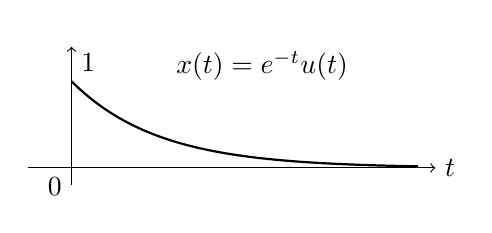
\begin{tikzpicture}[x=1.1cm,y=1.1cm]
\draw[->] (-0.5,0) -- (4.2,0) node[right] {$t$};
\draw[->] (0,-0.2) -- (0,1.4) node[above] {};
\node[below left] at (0,0) {0};
\draw[thick,domain=0:4,samples=60] plot (\x,{exp(-\x)});
\draw[dashed] (0,1) -- (0,0) node[below left] {};
\node[above right] at (0,1) {$1$};
\node[above] at (2.2,0.9) {$x(t)=e^{-t}u(t)$};
\end{tikzpicture}
\end{center}

	\textbf{Vraag:}
\begin{enumerate}[label=(\alph*)]
\item Bepaal $y_1(t) = x(t-2)$ (tijdsverschuiving).
\item Bepaal $y_2(t) = x(2t)$ (tijdscompressie).
\item Bepaal $y_3(t) = 2x(t)$ (amplitude schaling).
\item Schets alle drie signalen.
\end{enumerate}

\subsection{Oefening 2.6: Signaalenergie}

Bepaal de energie van de volgende signalen:

	\textbf{Vraag:}
\begin{enumerate}[label=(\alph*)]
\item $x(t) = e^{-t}u(t)$
\item $x(t) = 2\sin(t)u(t)$ over $0 \le t \le \pi$
\item $x(t) = \text{rect}(t) = u(t+0.5) - u(t-0.5)$
\end{enumerate}

\subsection{Oefening 2.7: Driehoeksignaal met Stapfuncties}

Definieer het signaal
\[
x(t) = t\big(u(t)-u(t-1)\big) + (2-t)\big(u(t-1)-u(t-2)\big).
\]

\begin{center}
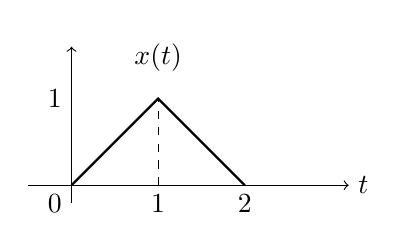
\begin{tikzpicture}[x=1.1cm,y=1.1cm]
\draw[->] (-0.5,0) -- (3.2,0) node[right] {$t$};
\draw[->] (0,-0.2) -- (0,1.6) node[above] {};
\node[below left] at (0,0) {0};
\draw[thick] (0,0) -- (1,1) -- (2,0);
\draw[dashed] (1,0) -- (1,1);
\node[below] at (1,0) {1};
\node[below] at (2,0) {2};
\node[left] at (0,1) {1};
\node[above] at (1,1.2) {$x(t)$};
\end{tikzpicture}
\end{center}


	\textbf{Vraag:}
\begin{enumerate}[label=(\alph*)]
\item Schrijf $x(t)$ expliciet als stukgewijze functie.
\item Bereken de energie $E = \int_{-\infty}^{\infty} |x(t)|^2\,dt$.
\item Bepaal en schets $x(t-1)$.
\end{enumerate}

\subsection{Oefening 2.8: Basis signaalbewerkingen (stapfunctie)}

Neem
\[
x(t)=u(t)-u(t-2).
\]

	\textbf{Vraag:}
\begin{enumerate}[label=(\alph*)]
\item Schets $x(t)$.
\item Schrijf $x(t-1)$ en $x(t+1)$ in termen van stapfuncties en schets ze.
\item Schrijf $x(2t)$ en $x(-t)$ in termen van stapfuncties en schets ze.
\end{enumerate}

\newpage

\section{Hoofdstuk 3: Laplacetransformatie}

\subsection{Oefening 3.1: Eenvoudige Laplacetransformaties}

Bepaal de Laplacetransformatie van de volgende functies:

\emph{Zie Formularium: definitie \ref{form:laplace-def} en paren \ref{form:laplace-pairs}.}

\textbf{Vraag:}
\begin{enumerate}[label=(\alph*)]
\item $f(t) = 5u(t)$
\item $f(t) = e^{-3t}u(t)$
\item $f(t) = t \cdot u(t)$
\item $f(t) = \cos(5t) \cdot u(t)$
\end{enumerate}

\subsection{Oefening 3.2: Inverse Laplacetransformatie}

Bepaal de inverse Laplacetransformatie van:
\[
F(s) = \frac{3}{s+2} + \frac{5}{s^2 + 4}
\]

\textbf{Vraag:} Vind $f(t)$.

\emph{Zie Formularium: paren \ref{form:laplace-pairs}.}

\subsection{Oefening 3.3: Eerste-Orde Systeem}

Los de volgende differentiaalvergelijking op met Laplacetransformatie:
\[
\frac{dy}{dt} + 4y = 8u(t), \quad y(0) = 2
\]

\textbf{Vraag:} Bepaal $y(t)$.

\emph{Zie Formularium: afgeleide-eigenschap \ref{form:laplace-prop}.}

\subsection{Oefening 3.4: Tweede-Orde Systeem}

Een massa-veer-dempersysteem wordt beschreven door:
\[
\frac{d^2y}{dt^2} + 4\frac{dy}{dt} + 3y = 0, \quad y(0) = 1, \quad y'(0) = 0
\]

\textbf{Vraag:}
\begin{enumerate}[label=(\alph*)]
\item Bepaal de karakteristieke vergelijking.
\item Vind de wortels van de karakteristieke vergelijking.
\item Los de differentiaalvergelijking op voor $y(t)$.
\end{enumerate}

\subsection{Oefening 3.5: Laplace-transformatie met Verschuiving}

Gegeven $F(s) = \frac{2}{s^2 + 4}$.

\textbf{Vraag:}
\begin{enumerate}[label=(\alph*)]
\item Bepaal $f(t) = \mathcal{L}^{-1}\{F(s)\}$.
\item Bepaal $g(t) = \mathcal{L}^{-1}\{e^{-2s}F(s)\}$ gebruikmakend van de tijdsverschuivingsstelling.
\end{enumerate}

\emph{Zie Formularium: tijdsverschuiving in $t$ \ref{form:laplace-prop}.}

\subsection{Oefening 3.6: Partieelbreuken}

Bepaal de inverse Laplacetransformatie van:
\[
F(s) = \frac{10}{(s+1)(s+2)(s+3)}
\]

\textbf{Vraag:} Bepaal $f(t)$ via partieelbreukontwikkeling.

\subsection{Oefening 3.7: Begin- en Eindwaardestelling}

Gegeven de functie in het s-domein:
\[
F(s) = \frac{3s + 5}{s^2 + 4s + 3}
\]

\textbf{Vraag:}
\begin{enumerate}[label=(\alph*)]
\item Bepaal de beginwaarde $f(0^+)$ met de beginwaardestelling.
\item Bepaal de eindwaarde $f(\infty)$ met de eindwaardestelling.
\item Controleer je antwoorden door $f(t)$ te berekenen.
\end{enumerate}

\emph{Zie Formularium: begin- en eindwaardestelling \ref{form:laplace-prop}.}

\subsection{Oefening 3.8: Convolutie via Laplace}

Gegeven
\[
f(t) = u(t) - u(t-1), \quad g(t) = e^{-2t}u(t).
\]
Definieer $y(t) = (f*g)(t)$.

\emph{Zie Formularium: convolutie-eigenschap \ref{form:laplace-prop}.}

	\textbf{Vraag:}
\begin{enumerate}[label=(\alph*)]
\item Bepaal $F(s)$ en $G(s)$.
\item Gebruik de convolutie-eigenschap in het $s$-domein om $Y(s)$ te vinden.
\item Bepaal $y(t)$ en geef het antwoord stukgewijs.
\end{enumerate}

\subsection{Oefening 3.9: Laplace}

	\textbf{Vraag:}
\begin{enumerate}[label=(\alph*)]
\item Bepaal $\mathcal{L}\{u(t)\}$.
\item Bepaal $\mathcal{L}\{e^{-2t}u(t)\}$.
\item Bepaal $\mathcal{L}\{t\,u(t)\}$.
\item Bepaal de inverse Laplace van $\displaystyle F(s)=\frac{1}{s+3}+\frac{2}{s^2}$.
\end{enumerate}

\newpage

\section{Hoofdstuk 4: Fouriertransformatie}

\subsection{Oefening 4.1: Fouriertransformatie van Rechthoekpuls}

Gegeven een rechthoekpuls:
\[
f(t) = \begin{cases}
A, & -T/2 < t < T/2 \\
0, & \text{elsewhere}
\end{cases}
\]

\begin{center}
\begin{tikzpicture}[x=1.2cm,y=1.2cm]
\draw[->] (-2.8,0) -- (2.8,0) node[right] {$t$};
\draw[->] (0,-0.2) -- (0,1.8) node[above] {};
\node[below left] at (0,0) {0};
\draw[thick] (-1.5,0) -- (-1.5,1.2) -- (1.5,1.2) -- (1.5,0);
\node[above] at (0,1.2) {$A$};
\node[below] at (-1.5,0) {$-T/2$};
\node[below] at (1.5,0) {$T/2$};
\end{tikzpicture}
\end{center}

\emph{Zie Formularium: blok $\leftrightarrow$ sinc in \ref{form:ft-pairs}.}

\textbf{Vraag:}
\begin{enumerate}[label=(\alph*)]
\item Bepaal de Fouriertransformatie $F(j\omega)$.
\item Schrijf het resultaat in de vorm van een sinc-functie.
\item Bepaal de eerste nulpunten van het spectrum.
\end{enumerate}

\subsection{Oefening 4.2: Verschuivingsstelling}

Gegeven $F\{f(t)\} = F(j\omega)$ bepaal de Fouriertransformatie van $f(t-t_0)$.

\emph{Zie Formularium: tijdverschuiving \ref{form:ft-prop}.}

\textbf{Vraag:}
\begin{enumerate}[label=(\alph*)]
\item Geef het bewijs van de verschuivingsstelling.
\item Pas deze toe op de puls uit oefening 4.1 met $t_0 = 1$ s, $A = 2$, $T = 2$ s.
\item Bespreek het effect op amplitude- en fasespectrum.
\end{enumerate}

\subsection{Oefening 4.3: Modulation Property}

Bepaal de Fouriertransformatie van het gemoduleerde signaal:
\[
x(t) = \cos(10\pi t) \cdot \text{rect}(t)
\]

waarbij $\text{rect}(t) = u(t+1) - u(t-1)$ is.

\emph{Zie Formularium: modulatie (cosinus) in \ref{form:ft-pairs}.}

\textbf{Vraag:}
\begin{enumerate}[label=(\alph*)]
\item Pas de modulatiestelling toe.
\item Schets het amplitude- en fasespectrum.
\end{enumerate}

\subsection{Oefening 4.4: Parseval's Stelling}

De energiedichtheid van een signaal wordt gegeven door Parseval's stelling. Gegeven $f(t) = e^{-t}u(t)$.

\emph{Zie Formularium: FTC-definitie \ref{form:ft-def} en eigenschappen \ref{form:ft-prop}.}

\textbf{Vraag:}
\begin{enumerate}[label=(\alph*)]
\item Bepaal de totale energie in het tijdsdomein: $E = \int_{-\infty}^{\infty} |f(t)|^2 dt$.
\item Bepaal $F(j\omega)$ en controleer de energie in het frequentiedomein.
\item Verifieer Parseval's stelling.
\end{enumerate}

\subsection{Oefening 4.5: Exponentieel Signaal}

Gegeven $f(t) = e^{-a|t|}$ met $a > 0$.

\textbf{Vraag:}
\begin{enumerate}[label=(\alph*)]
\item Bepaal de Fouriertransformatie $F(j\omega)$.
\item Schets het amplitude- en fasespectrum.
\item Bepaal de bandbreedte (eerste nulpunt).
\end{enumerate}

\subsection{Oefening 4.6: Dirac Delta}

Bepaal de Fouriertransformatie van:

\textbf{Vraag:}
\begin{enumerate}[label=(\alph*)]
\item $f(t) = \delta(t)$ (impulsfunctie)
\item $f(t) = \delta(t-t_0)$ (verschoven impulsfunctie)
\item $f(t) = \cos(\omega_0 t)$ (hint: gebruik dat $\cos(\omega_0 t) = \frac{1}{2}(e^{j\omega_0 t} + e^{-j\omega_0 t})$)
\end{enumerate}

\subsection{Oefening 4.7: Verschuiving in de Tijd (FTC)}

Beschouw het bloksignaal
\[
x(t) = \begin{cases}
2, & -\tfrac{1}{2} < t < \tfrac{1}{2}\\
0, & \text{elsewhere}
\end{cases}
\]
en definieer $y(t) = x(t-t_0)$ met $t_0 = \tfrac{1}{4}$.

	\textbf{Vraag:}
\begin{enumerate}[label=(\alph*)]
\item Bepaal $X(j\omega)$.
\item Bepaal $Y(j\omega)$ met de verschuivingsstelling en bespreek het effect op fase en amplitude.
\end{enumerate}

\subsection{Oefening 4.8: FTC van delta's}

Gebruik de bekende paren $\mathcal{F}\{\delta(t)\}=1$ en de verschuivingsstelling.

	\textbf{Vraag:}
\begin{enumerate}[label=(\alph*)]
\item Bepaal $\mathcal{F}\{\delta(t-t_0)\}$.
\item Bepaal de Fouriertransformatie van $x(t)=2\delta(t)-\delta(t-1)$.
\item Wat is het amplitudespectrum van $x(t)$ uit (b)? (geen volledige schets nodig)
\end{enumerate}

\newpage

\section{Hoofdstuk 5: Fourierreeksen}

\subsection{Oefening 5.1: Blokgolf}

Een periodieke blokgolf met periode $T = 2$ s is gedefinieerd als:
\[
f(t) = \begin{cases}
1, & 0 < t < 1 \\
-1, & 1 < t < 2
\end{cases}
\]

\begin{center}
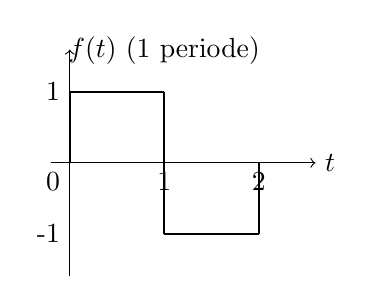
\begin{tikzpicture}[x=1.2cm,y=0.9cm]
\draw[->] (-0.2,0) -- (2.6,0) node[right] {$t$};
\draw[->] (0,-1.6) -- (0,1.6) node[above] {};
\node[below left] at (0,0) {0};
\draw[thick] (0,1) -- (1,1);
\draw[thick] (1,-1) -- (2,-1);
\draw[thick] (0,1) -- (0,0);
\draw[thick] (1,1) -- (1,-1);
\draw[thick] (2,-1) -- (2,0);
\node[below] at (1,0) {1};
\node[below] at (2,0) {2};
\node[left] at (0,1) {1};
\node[left] at (0,-1) {-1};
\node[above] at (1,1.25) {$f(t)$ (1 periode)};
\end{tikzpicture}
\end{center}

\emph{Zie Formularium: Fourierreeks (cartesisch) \ref{form:fs-cart} en (complex) \ref{form:fs-cplx}.}

\textbf{Vraag:}
\begin{enumerate}[label=(\alph*)]
\item Bepaal of de functie even, oneven, of geen van beide is.
\item Bereken de Fourierco\"effici\"enten $a_0$, $a_n$, en $b_n$.
\item Schrijf de Fourierreeks tot de 3e harmonische.
\end{enumerate}

\subsection{Oefening 5.2: Zaagtandgolf}

Een zaagtandgolf met periode $T = 1$ s is gegeven door $f(t) = 2t$ voor $0 < t < 1$.

\begin{center}
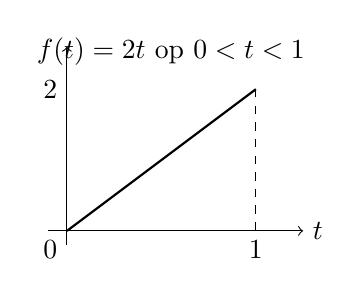
\begin{tikzpicture}[x=2.4cm,y=0.9cm]
\draw[->] (-0.1,0) -- (1.25,0) node[right] {$t$};
\draw[->] (0,-0.2) -- (0,2.6) node[above] {};
\node[below left] at (0,0) {0};
\draw[thick] (0,0) -- (1,2);
\draw[dashed] (1,2) -- (1,0);
\node[below] at (1,0) {1};
\node[left] at (0,2) {2};
\node[above] at (0.55,2.2) {$f(t)=2t$ op $0<t<1$};
\end{tikzpicture}
\end{center}

\textbf{Vraag:}
\begin{enumerate}[label=(\alph*)]
\item Bereken $a_0$.
\item Bepaal $b_1$ en $b_2$.
\item Schrijf de benaderende Fouriersom met 2 termen.
\end{enumerate}

\subsection{Oefening 5.3: Driehoekgolf}

Een driehoekgolf met periode $T = 2$ is gedefinieerd als:
\[
f(t) = \begin{cases}
t, & 0 \le t < 1 \\
2-t, & 1 \le t < 2
\end{cases}
\]

\textbf{Vraag:}
\begin{enumerate}[label=(\alph*)]
\item Is dit signaal even of oneven?
\item Bepaal de Fourierco\"effici\"enten.
\item Schrijf de eerste drie niet-nul termen van de Fourierreeks.
\end{enumerate}

\subsection{Oefening 5.4: Parseval's Stelling voor Fourierreeksen}

Gegeven de blokgolf uit oefening 5.1.

\textbf{Vraag:}
\begin{enumerate}[label=(\alph*)]
\item Bereken de gemiddelde macht van het signaal: $P = \frac{1}{T}\int_0^T f^2(t) dt$.
\item Bereken $P$ uit de Fourierco\"effici\"enten met Parseval's stelling: $P = a_0^2 + \frac{1}{2}\sum_{n=1}^{\infty} (a_n^2 + b_n^2)$.
\item Controleer dat beide methoden dezelfde waarde geven.
\end{enumerate}

\subsection{Oefening 5.5: Complexe Fourierreeks en Link met FTC}

Definieer een periodiek signaal met periode $T=2$ als
\[
f(t) = \begin{cases}
1, & 0 < t < 1 \\
0, & 1 < t < 2
\end{cases}
\quad \text{en periodiek uitgebreid.}
\]

	\textbf{Vraag:}
\begin{enumerate}[label=(\alph*)]
\item Bepaal de complexe Fourierco\"effici\"enten $c_k$ (met $\omega_0 = 2\pi/T$).
\item Geef een eenvoudige interpretatie van welke harmonischen verdwijnen.
\item Gebruik de link uit het formularium $X(k\omega_0)=T\,c_k$ om uit te leggen hoe de FTC van \emph{\'e\'en periode} gesampled wordt.
\end{enumerate}

\subsection{Oefening 5.6: Fourierreeks van een eenvoudige som}

Neem een periodiek signaal met periode $T=2\pi$:
\[
f(t)=\sin(t)+2\cos(2t).
\]

	\textbf{Vraag:}
\begin{enumerate}[label=(\alph*)]
\item Geef $\omega_0$.
\item Bepaal de re\"ele Fourierco\"effici\"enten $a_0$, $a_n$ en $b_n$.
\item Schrijf de Fourierreeks expliciet (je mag meteen herkennen welke termen niet nul zijn).
\end{enumerate}

\newpage

\section{Hoofdstuk 6: LTC-Systemen}

\subsection{Oefening 6.1: Impulsrespons}

Een eerste-orde systeem heeft impulsrespons $h(t) = 2e^{-5t}u(t)$.

\begin{center}
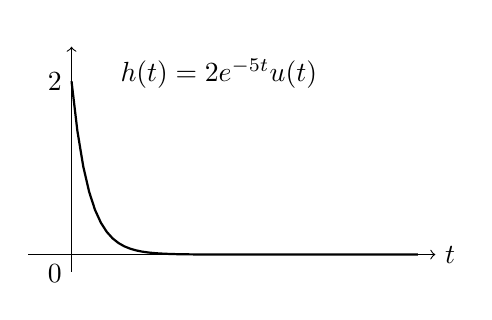
\begin{tikzpicture}[x=1.1cm,y=1.1cm]
\draw[->] (-0.5,0) -- (4.2,0) node[right] {$t$};
\draw[->] (0,-0.2) -- (0,2.4) node[above] {};
\node[below left] at (0,0) {0};
\draw[thick,domain=0:4,samples=60] plot (\x,{2*exp(-5*\x)});
\node[above] at (1.7,1.8) {$h(t)=2e^{-5t}u(t)$};
\node[left] at (0,2) {2};
\end{tikzpicture}
\end{center}

\textbf{Vraag:}
\begin{enumerate}[label=(\alph*)]
\item Bereken de systeemrespons op een stapingang $f(t) = u(t)$ door convolutie.
\item Verifieer je antwoord met de Laplacetransformatie.
\end{enumerate}

\subsection{Oefening 6.2: Massa-Veer-Demper}

Een massa-veer-dempersysteem heeft $m = 2$ kg, $k = 8$ N/m, en $c = 4$ Ns/m.

\textbf{Vraag:}
\begin{enumerate}[label=(\alph*)]
\item Schrijf de differentiaalvergelijking.
\item Bepaal de natuurlijke eigenfrequentie $\omega_0$.
\item Is het systeem ondergedempt, kritisch gedempt, of overgedempt?
\end{enumerate}

\subsection{Oefening 6.3: Frequentierespons}

Gegeven een LTC-systeem met overdracht $H(s) = \frac{10}{s+5}$.

\textbf{Vraag:}
\begin{enumerate}[label=(\alph*)]
\item Bepaal de frequentierespons $H(j\omega)$.
\item Bepaal de amplitude- en faserespons.
\item Bepaal de 3dB bandbreedte (waar $|H(j\omega)| = \frac{|H(0)|}{\sqrt{2}}$).
\end{enumerate}

\subsection{Oefening 6.4: Cascade Systemen}

Gegeven twee LTC-systemen in cascade:
\[
H_1(s) = \frac{5}{s+2}, \quad H_2(s) = \frac{3}{s+3}
\]

\textbf{Vraag:}
\begin{enumerate}[label=(\alph*)]
\item Bepaal de totale overdracht $H(s) = H_1(s) \cdot H_2(s)$.
\item Bepaal de impulsrespons $h(t) = \mathcal{L}^{-1}\{H(s)\}$.
\end{enumerate}

\subsection{Oefening 6.5: Stabiliteit en Polen}

Bepaal voor de volgende systemen of ze BIBO-stabiel, marginaal stabiel of onstabiel zijn op basis van hun polen.

\textbf{Vraag:}
\begin{enumerate}[label=(\alph*)]
\item $H_1(s) = \frac{1}{s-2}$
\item $H_2(s) = \frac{1}{s^2+3s+2}$
\item $H_3(s) = \frac{1}{s^2+4}$
\end{enumerate}

\subsection{Oefening 6.6: Overdracht, Impulsrespons en Nultoestandsrespons}

Een LTC-systeem voldoet aan de differentiaalvergelijking (met nul beginvoorwaarden)
\[
\frac{dy}{dt} + 3y(t) = x(t).
\]

	\textbf{Vraag:}
\begin{enumerate}[label=(\alph*)]
\item Bepaal de overdrachtsfunctie $H(s)=\frac{Y(s)}{X(s)}$.
\item Bepaal de impulsrespons $h(t)$.
\item Is het systeem BIBO-stabiel? Motiveer via de polen.
\item Bepaal de nultoestandsrespons $y(t)$ voor $x(t)=u(t)-u(t-1)$.
\end{enumerate}

\subsection{Oefening 6.7: Impuls- en staprespons (basis)}

Een causaal LTC-systeem heeft overdracht
\[
H(s)=\frac{1}{s+1}.
\]

	\textbf{Vraag:}
\begin{enumerate}[label=(\alph*)]
\item Bepaal de impulsrespons $h(t)$.
\item Bepaal de staprespons $y(t)$ voor $x(t)=u(t)$.
\item Wat is de tijdsconstante $\tau$ en de DC-versterking $H(0)$?
\end{enumerate}

\newpage

\section{Hoofdstuk 7: Eigenwaarden en Eigenvectoren}

\subsection{Oefening 7.1: Eigenwaarden Berekenen}

Gegeven de matrix:
\[
A = \begin{pmatrix} 4 & 1 \\ 2 & 3 \end{pmatrix}
\]

\textbf{Vraag:}
\begin{enumerate}[label=(\alph*)]
\item Bepaal de karakteristieke veelterm $f(\lambda) = |A - \lambda I|$.
\item Vind de eigenwaarden van $A$.
\item Bereken voor elke eigenwaarde een bijbehorende eigenvector.
\end{enumerate}

\subsection{Oefening 7.2: Eigenwaarden van Tweede-Orde Systeem}

Voor het systeem uit oefening 3.4 ($\frac{d^2y}{dt^2} + 4\frac{dy}{dt} + 3y = 0$).

\textbf{Vraag:}
\begin{enumerate}[label=(\alph*)]
\item Schrijf dit differentiaalvergelijkingssysteem als een eerste-orde matrixvergelijking:
\[
\frac{d}{dt}\begin{pmatrix} y \\ \dot{y} \end{pmatrix} = \begin{pmatrix} 0 & 1 \\ -3 & -4 \end{pmatrix} \begin{pmatrix} y \\ \dot{y} \end{pmatrix}
\]
\item Bepaal de eigenwaarden van deze systeemmatrix.
\item Verifieer dat dit overeenkomt met de karakteristieke vergelijking uit oefening 3.4.
\item Bepaal de eigenvectoren.
\end{enumerate}

\subsection{Oefening 7.3: Diagonalisatie}

Gegeven de matrix:
\[
A = \begin{pmatrix} 5 & -2 \\ -2 & 2 \end{pmatrix}
\]

\textbf{Vraag:}
\begin{enumerate}[label=(\alph*)]
\item Bepaal alle eigenwaarden en bijbehorende eigenvectoren.
\item Controleer dat de eigenvectoren orthogonaal zijn (omdat $A$ symmetrisch is).
\item Vorm de matrix $P$ met eigenvectoren als kolommen en bepaal $P^{-1}AP = D$ waarbij $D$ diagonaal is.
\end{enumerate}

\subsection{Oefening 7.4: Gerschgorin-Cirkelstelling}

Gegeven de matrix:
\[
A = \begin{pmatrix} 4 & 0.5 & 0.2 \\ 0.3 & -2 & 0.1 \\ 0.2 & 0.4 & 3 \end{pmatrix}
\]

\textbf{Vraag:}
\begin{enumerate}[label=(\alph*)]
\item Bepaal de Gerschgorin-cirkels voor deze matrix.
\item Geef grenzen voor de eigenwaarden op basis van de stelling.
\item Bepaal de eigenwaarden numeriek en controleer of ze binnen de cirkels vallen.
\end{enumerate}

\subsection{Oefening 7.5: Eigenvectoren en Orthogonaliteit}

Gegeven de matrix:
\[
B = \begin{pmatrix} 3 & 1 \\ 1 & 3 \end{pmatrix}
\]

\textbf{Vraag:}
\begin{enumerate}[label=(\alph*)]
\item Bepaal de eigenwaarden.
\item Bepaal de eigenvectoren.
\item Toon aan dat de eigenvectoren orthogonaal zijn.
\item Normaliseer de eigenvectoren tot eenheid.
\end{enumerate}

\subsection{Oefening 7.6: Matrix Exponenti\"ele}

Gegeven de matrix $A = \begin{pmatrix} 0 & 1 \\ -2 & -3 \end{pmatrix}$.

\textbf{Vraag:}
\begin{enumerate}[label=(\alph*)]
\item Bepaal de eigenwaarden en eigenvectoren van $A$.
\item Bereken de matrix exponenti\"ele $e^{At}$ via diagonalisatie of Cayley-Hamilton.
\item Gebruik dit om de oplossing van $\dot{\mathbf{x}} = A\mathbf{x}$ te vinden met $\mathbf{x}(0) = \begin{pmatrix} 1 \\ 0 \end{pmatrix}$.
\end{enumerate}

\subsection{Oefening 7.7: Niet-diagonaliseerbaar en Matrixexponentiaal}

Gegeven
\[
A = \begin{pmatrix} 2 & 1 \\ 0 & 2 \end{pmatrix}.
\]


	\textbf{Vraag:}
\begin{enumerate}[label=(\alph*)]
\item Bepaal de eigenwaarden van $A$ en de dimensie van de eigenruimte.
\item Is $A$ diagonaliseerbaar? Motiveer.
\item Bepaal $e^{At}$.
\end{enumerate}

\subsection{Oefening 7.8: Eigenwaarden van een diagonaalmatrix (basis)}

Gegeven
\[
A=\begin{pmatrix}1 & 0\\ 0 & 2\end{pmatrix}.
\]

	\textbf{Vraag:}
\begin{enumerate}[label=(\alph*)]
\item Bepaal de eigenwaarden en geef voor elke eigenwaarde een eigenvector.
\item Bereken $A^3$.
\item Bereken $e^{At}$.
\end{enumerate}

\newpage

\section{Hoofdstuk 8: Examengerichte Oefeningen}

\subsection{Oefening 8.1: FTC-eigenschappen (Verschuiving en Modulatie)}

Definieer het bloksignaal
\[
x(t) = \begin{cases}
1, & -\tfrac{1}{2}<t<\tfrac{1}{2}\\
0, & \text{elsewhere}
\end{cases}
\]
en de cosinus $v(t)=2\cos(2\pi t)$. Definieer $y(t)=x(t)\cos(2\pi t)$ en $z(t)=x(t)+x(t-1)$.

	\textbf{Vraag:}
\begin{enumerate}[label=(\alph*)]
\item Welke van de signalen $x(t)$, $v(t)$, $y(t)$ en $z(t)$ zijn even/oneven?
\item Bepaal $Y(j\omega)$ met de modulatiestelling en een gekende FTC-paar voor $x(t)$.
\item Bepaal $Z(j\omega)$ met de verschuivingsstelling.
\end{enumerate}

\subsection{Oefening 8.2: Laplace, Causaliteit en Convolutie}

Het ingangssignaal is $x(t)=u(t)-u(t-2)$ en de impulsrespons is $h(t)=e^{-t}u(t)$.

\begin{center}
\begin{tikzpicture}[x=1.0cm,y=1.0cm]
\draw[->] (-0.5,0) -- (4.2,0) node[right] {$t$};
\draw[->] (0,-0.2) -- (0,1.6) node[above] {};
\node[below left] at (0,0) {0};
% x(t)
\draw[thick] (0,0) -- (0,1) -- (2,1) -- (2,0);
\node[above] at (1,1) {$x(t)$};
\node[below] at (2,0) {2};
\end{tikzpicture}
\end{center}

	\textbf{Vraag:}
\begin{enumerate}[label=(\alph*)]
\item Bepaal $X(s)$.
\item Is het systeem causaal? Motiveer op basis van $h(t)$.
\item Bepaal $y(t)=h(t)*x(t)$ en geef het antwoord stukgewijs.
\end{enumerate}

\subsection{Oefening 8.3: Complexe Fourierreeks (Puls-trein)}

Definieer een periodiek signaal met periode $T=2$ als
\[
p(t)=\begin{cases}
1, & 0<t<\tfrac{1}{2}\\
0, & \tfrac{1}{2}<t<2
\end{cases}
\quad \text{en periodiek uitgebreid.}
\]

	\textbf{Vraag:}
\begin{enumerate}[label=(\alph*)]
\item Bepaal de complexe Fourierco\"effici\"enten $c_k$.
\item Welke symmetrie zie je in $c_{-k}$ t.o.v. $c_k$ als $p(t)$ re\"eel is?
\item (Extra) Gebruik opnieuw de link $X(k\omega_0)=T\,c_k$ om te interpreteren wat de harmonischen betekenen in het frequentiedomein.
\end{enumerate}

\subsection{Oefening 8.4: Laplace met verschuiving en initieelwaarden}

Beschouw
\[
x(t)=e^{-t}u(t)-e^{-(t-2)}u(t-2).
\]

	\textbf{Vraag:}
\begin{enumerate}[label=(\alph*)]
\item Bepaal $X(s)$.
\item Bepaal $x(0^+)$ en $\lim_{t\to\infty}x(t)$ rechtstreeks uit $x(t)$.
\item Verifieer $x(0^+)$ met de beginwaardestelling en $\lim_{t\to\infty}x(t)$ met de eindwaardestelling (als toepasbaar).
\end{enumerate}

\subsection{Oefening 8.5: Differentiaalvergelijking (Laplace, stapinput)}

Gegeven
\[
y''(t)+3y'(t)+2y(t)=u(t),\qquad y(0)=0,\quad y'(0)=1.
\]

	\textbf{Vraag:}
\begin{enumerate}[label=(\alph*)]
\item Los $y(t)$ op met de (unilaterale) Laplace-transformatie.
\item Geef $y(t)$ stukgewijs (indien nodig) en vereenvoudig maximaal.
\end{enumerate}

\subsection{Oefening 8.6: LTI-systeem (polen, stabiliteit, staprespons)}

Een causaal LTI-systeem heeft
\[
H(s)=\frac{s+2}{s(s+4)}.
\]

	\textbf{Vraag:}
\begin{enumerate}[label=(\alph*)]
\item Bepaal $h(t)$.
\item Is het systeem BIBO-stabiel? Motiveer.
\item Bepaal de staprespons $y(t)$ voor $x(t)=u(t)$.
\item Bepaal $\lim_{t\to\infty}y(t)$ en controleer met de eindwaardestelling.
\end{enumerate}

\subsection{Oefening 8.7: Convolutie + Laplace-check}

Neem $x(t)=u(t)-u(t-1)$ en $h(t)=t\,u(t)$.

	\textbf{Vraag:}
\begin{enumerate}[label=(\alph*)]
\item Bepaal $y(t)=(x*h)(t)$ via convolutie in het tijdsdomein en geef het resultaat stukgewijs.
\item Controleer je antwoord door Laplace: $Y(s)=X(s)H(s)$ en inverse Laplace.
\end{enumerate}

\subsection{Oefening 8.8: Fouriertransformatie + Parseval (energie)}

Voor $a>0$:
\[
x(t)=e^{-a|t|}.
\]

	\textbf{Vraag:}
\begin{enumerate}[label=(\alph*)]
\item Bepaal $X(j\omega)$.
\item Bereken de energie $E=\int_{-\infty}^{\infty}|x(t)|^2\,dt$.
\item Controleer met Parseval.
\end{enumerate}

\subsection{Oefening 8.9: Re\"ele Fourierreeks (symmetrie + RMS)}

Definieer een periodiek signaal met periode $T=2\pi$:
\[
f(t)=\begin{cases}
1, & 0<t<\pi\\
-1, & -\pi<t<0
\end{cases}
\quad \text{en periodiek uitgebreid.}
\]

	\textbf{Vraag:}
\begin{enumerate}[label=(\alph*)]
\item Geef aan of $f(t)$ even/oneven is.
\item Bepaal de re\"ele Fourierreeks van $f(t)$.
\item Bepaal de RMS-waarde van $f(t)$ en verifieer met Parseval (reeks-vorm).
\end{enumerate}

\subsection{Oefening 8.10: Toestandruimte en eigenwaarden (stabiliteit + oplossing)}

Beschouw het systeem
\[
\dot{\mathbf{x}}=A\mathbf{x},\qquad
A=\begin{pmatrix}0 & 1\\ -2 & -3\end{pmatrix},\qquad \mathbf{x}(0)=\begin{pmatrix}1\\0\end{pmatrix}.
\]

	\textbf{Vraag:}
\begin{enumerate}[label=(\alph*)]
\item Bepaal de eigenwaarden van $A$ en bespreek de stabiliteit van de oorsprong.
\item Bepaal $\mathbf{x}(t)$ expliciet (via diagonalisatie of via oplossing van een tweede-orde vergelijking).
\item Geef ook $x_1(t)$ en $x_2(t)$ afzonderlijk.
\end{enumerate}

\subsection{Oefening 8.11: Impulsrespons en Stabiliteit met Polen}

Gegeven een causaal LTC-systeem met overdrachtsfunctie
\[
H(s) = \frac{2s + 3}{s^2 + 5s + 6}.
\]

\emph{Bron: Oefeningenbundel 25–26 (thema Laplace en LTI-systemen).}

\textbf{Vraag:}
\begin{enumerate}[label=(\alph*)]
\item Bepaal de polen van het systeem.
\item Onderzoek BIBO-stabiliteit op basis van de poollocaties.
\item Bepaal de impulsrespons $h(t) = \mathcal{L}^{-1}\{H(s)\}$ via partieelbreuken.
\item Bepaal de staprespons voor $x(t) = u(t)$.
\end{enumerate}

\subsection{Oefening 8.12: Differentiaalvergelijking uit Overdrachtsfunctie}

Een LTC-systeem wordt beschreven door de overdrachtsfunctie
\[
H(s) = \frac{Y(s)}{X(s)} = \frac{4}{s^2 + 3s + 2}.
\]

\emph{Bron: Oefeningenbundel 25–26 (thema differentiaalvergelijkingen en Laplace).}

\textbf{Vraag:}
\begin{enumerate}[label=(\alph*)]
\item Bepaal de differentiaalvergelijking die het systeem beschrijft.
\item Los deze differentiaalvergelijking op (homogeen + particulier) voor input $x(t) = 2u(t)$ met beginvoorwaarden $y(0) = 0$ en $y'(0) = 1$.
\item Controleer je antwoord met de Laplacetransformatie.
\end{enumerate}

\subsection{Oefening 8.13: Fouriertransformatie van Exponentieel Signaal}

Gegeven het signaal
\[
f(t) = 3e^{-2t}u(t).
\]

\emph{Bron: Oefeningenbundel 25–26 (Fouriertransformatie en energieanalyse).}

\textbf{Vraag:}
\begin{enumerate}[label=(\alph*)]
\item Bepaal de Fouriertransformatie $F(j\omega)$ (gebruik de link met Laplace).
\item Bepaal en schets het amplitudespectrum $|F(j\omega)|$.
\item Bereken de energiedichtheid $E = \int_{-\infty}^{\infty} |f(t)|^2 dt$.
\item Verifieer Parseval's stelling: $E = \frac{1}{2\pi}\int_{-\infty}^{\infty} |F(j\omega)|^2 d\omega$.
\end{enumerate}

\newpage

\section{Oplossingen}

\subsection{Oplossingen Hoofdstuk 1}

\subsubsection*{Oplossing 1.1}

\textbf{Gegeven:} Systeem met operator $\mathcal{T}\{x(t)\} = 3x(t) + 2$.

\textbf{Vraag:} Onderzoek of dit systeem lineair is.

\textbf{Oplossing:}

\begin{itemize}
\item Test eigenschap 1 (schaling): $\mathcal{T}\{ax(t)\} = 3ax(t) + 2 \neq a\mathcal{T}\{x(t)\} = a(3x(t) + 2) = 3ax(t) + 2a$
\item Voor $a \neq 1$ geldt: $2 \neq 2a$, dus schaling klopt niet.
\item Omdat de schalingsvoorwaarde niet voldaan is, is het systeem niet lineair.
\end{itemize}

\subsubsection*{Oplossing 1.2}

\textbf{Gegeven:} RC-circuit met $R = 1000$ $\Omega$, $C = 10$ $\mu$F, ingangsspanning $v_{\text{in}}(t) = 5u(t)$ V.

\textbf{Vraag:} 
\begin{enumerate}[label=(\alph*)]
\item Schrijf de differentiaalvergelijking op.
\item Bereken $\tau$.
\item Bepaal $v_{\text{uit}}(0.01)$.
\end{enumerate}

\textbf{Oplossing:}

\begin{enumerate}[label=(\alph*)]
\item De differentiaalvergelijking van een RC-circuit: $RC\frac{dv_{\text{uit}}}{dt} + v_{\text{uit}} = v_{\text{in}}$

\[
(1000)(10 \times 10^{-6})\frac{dv_{\text{uit}}}{dt} + v_{\text{uit}} = 5u(t)
\]

\[
0.01\frac{dv_{\text{uit}}}{dt} + v_{\text{uit}} = 5u(t)
\]

\item Tijdsconstante: $\tau = RC = (1000)(10 \times 10^{-6}) = 0.01$ s $= 10$ ms

\item Voor een staprespons met $v_{\text{uit}}(0) = 0$:

\[
v_{\text{uit}}(t) = 5(1 - e^{-t/\tau})u(t) = 5(1 - e^{-100t})u(t)
\]

Op $t = 10$ ms $= 0.01$ s:

\[
v_{\text{uit}}(0.01) = 5(1 - e^{-1}) = 5(1 - 0.368) = 5(0.632) = 3.16 \text{ V}
\]
\end{enumerate}

\subsubsection*{Oplossing 1.3}

			\textbf{Gegeven:} Radio-isotoop met halveringstijd $t_{1/2} = 6$ uur. Initi\"ele hoeveelheid: 20 mg om 08:00.

\textbf{Vraag:} Hoeveel mg blijft over om 14:00?

\textbf{Oplossing:}

Model radioactief verval: $N(t) = N_0 e^{-kt}$

Halveringstijd $t_{1/2} = 6$ uur: $\frac{1}{2} = e^{-6k} \Rightarrow k = \frac{\ln(2)}{6} = 0.1155$ h$^{-1}$

Van 08:00 tot 14:00 is $\Delta t = 6$ uur:

\[
N(6) = 20 e^{-0.1155 \times 6} = 20 e^{-0.693} = 20 \times 0.5 = 10 \text{ mg}
\]

\textbf{Antwoord:} 10 mg blijft over.

\subsubsection*{Oplossing 1.4}

\textbf{Gegeven:} Twee systemen:
- Systeem A: $\mathcal{T}\{x(t)\} = 2x(t)$
- Systeem B: $\mathcal{T}\{x(t)\} = x(t) + 1$

\textbf{Vraag:} Test op homogeniteit en additiviteit; bepaal lineariteit.

\textbf{Oplossing:}

\textbf{Systeem A: } $\mathcal{T}\{x(t)\} = 2x(t)$

Homogeniteit: $\mathcal{T}\{ax(t)\} = 2ax(t) = a(2x(t)) = a\mathcal{T}\{x(t)\}$ \checkmark

Additiviteit: $\mathcal{T}\{x_1(t) + x_2(t)\} = 2(x_1(t) + x_2(t)) = 2x_1(t) + 2x_2(t) = \mathcal{T}\{x_1(t)\} + \mathcal{T}\{x_2(t)\}$ \checkmark

\textbf{Systeem A is LINEAIR.}

\textbf{Systeem B: } $\mathcal{T}\{x(t)\} = x(t) + 1$

Homogeniteit: $\mathcal{T}\{ax(t)\} = ax(t) + 1 \neq a(x(t) + 1) = ax(t) + a = a\mathcal{T}\{x(t)\}$ (voor $a \neq 1$) \text{\sffamily X}

\textbf{Systeem B is NIET LINEAIR.}

\subsubsection*{Oplossing 1.5}

\textbf{Gegeven:} Vier systemen. 
\textbf{Vraag:} Welke zijn LTI?

\textbf{Oplossing:}

\begin{enumerate}[label=(\alph*)]
\item $y(t) = x(t-2)$: LINEAIR en TIJDINVARIANT \checkmark (zuivere vertraging)

\item $y(t) = tx(t)$: LINEAIR maar NIET TIJDINVARIANT \text{\sffamily X} (co\"effici\"ent varieert in tijd)

\item $y(t) = |x(t)|$: NIET LINEAIR \text{\sffamily X} (niet additief/homogeen)

\item $y(t) = \int_0^t x(\tau) d\tau$: LINEAIR en TIJDINVARIANT \checkmark (integrator)

\end{enumerate}

\textbf{Antwoord:} (a) en (d) zijn LTI.

\subsubsection*{Oplossing 1.6}

	\textbf{Gegeven:} $y(t)=x(t)+x(t-1)$.

	\textbf{Vraag:} Onderzoek lineariteit/tijdinvariantie; causaliteit; invertibiliteit.

	\textbf{Oplossing:}
\begin{enumerate}[label=(\alph*)]
\item \textbf{Lineair en tijdinvariant:} Het systeem is lineair (som van lineaire operatoren) en tijdinvariant omdat een tijdsverschuiving van de input dezelfde verschuiving in beide termen geeft.
\item \textbf{Causaal:} Ja. $y(t)$ hangt af van $x(t)$ en $x(t-1)$, dus enkel van huidige en verleden waarden.
\item \textbf{Invertibel:} \textbf{Niet} uniek invertibel.

\textbf{Bewijs door tegenvoorbeeld:}

Stel $y(t) = 0$ voor alle $t$. Dan geldt:
\[
x(t) + x(t-1) = 0 \Rightarrow x(t) = -x(t-1)
\]

Deze vergelijking heeft oneindig veel oplossingen, bijvoorbeeld:
\begin{itemize}
\item $x(t) = A(-1)^t$ voor elke constante $A$
\item $x(t) = 0$ voor alle $t$
\end{itemize}

Omdat verschillende inputs tot dezelfde output leiden, is het systeem niet invertibel.
\end{enumerate}

\subsubsection*{Oplossing 1.7}

	\textbf{Gegeven:} (S1) $y(t)=2x(t-1)$ en (S2) $y(t)=x(t)+u(t)$.

	\textbf{Vraag:} Onderzoek lineariteit, tijdinvariantie en causaliteit voor (S1) en (S2).

	\textbf{Oplossing:}

\begin{enumerate}[label=(\alph*)]
\item \textbf{Lineariteit}

\textbf{Systeem (S1): $y(t)=2x(t-1)$}

\textbf{Test homogeniteit:} Voor $ax(t)$:
\[
\mathcal{T}\{ax(t)\} = 2ax(t-1) = a\cdot 2x(t-1) = a\mathcal{T}\{x(t)\} \quad \checkmark
\]

\textbf{Test additiviteit:} Voor $x_1(t) + x_2(t)$:
\[
\mathcal{T}\{x_1(t)+x_2(t)\} = 2(x_1(t-1)+x_2(t-1)) = 2x_1(t-1) + 2x_2(t-1) = \mathcal{T}\{x_1(t)\} + \mathcal{T}\{x_2(t)\} \quad \checkmark
\]

$\Rightarrow$ (S1) is \textbf{lineair}.

\textbf{Systeem (S2): $y(t)=x(t)+u(t)$}

\textbf{Nultoestandtest:} Voor $x(t)=0$:
\[
\mathcal{T}\{0\} = 0 + u(t) = u(t) \neq 0
\]

Dit schendt het nultoestandcriterium voor lineariteit.

$\Rightarrow$ (S2) is \textbf{niet lineair}.

\item \textbf{Tijdinvariantie}
\begin{itemize}
\item (S1) is \textbf{tijdinvariant}: $x(t)\mapsto x(t-t_0)$ geeft $y(t)=2x(t-1)\mapsto 2x(t-t_0-1)=y(t-t_0)$.
\item (S2) is \textbf{niet tijdinvariant}: voor $x(t)$ is $y(t)=x(t)+u(t)$. Voor $x(t-t_0)$ is de output $x(t-t_0)+u(t)$, terwijl $y(t-t_0)=x(t-t_0)+u(t-t_0)$. Niet gelijk als $t_0\neq 0$.
\end{itemize}

\item \textbf{Causaliteit}
\begin{itemize}
\item (S1) is \textbf{causaal}: $y(t)$ hangt af van $x(t-1)$ (verleden).
\item (S2) is \textbf{causaal}: $y(t)$ hangt af van $x(t)$ en een gekend signaal $u(t)$.
\end{itemize}
\end{enumerate}

\subsection{Oplossingen Hoofdstuk 2}

\subsubsection*{Oplossing 2.1}

\textbf{Gegeven:} $x_1(t) = e^{0.2t}$ en $x_2(t) = e^{-0.5t}$.

\textbf{Vraag:} Bepaal welk signaal exponenti\"ele groei/verval vertoont; bereken waarden op $t = 5$ s.

\textbf{Oplossing:}

\begin{enumerate}[label=(\alph*)]
\item $x_1(t) = e^{0.2t}$: exponenti\"ele \textbf{groei} (positieve exponent)
$x_2(t) = e^{-0.5t}$: exponentieel \textbf{verval} (negatieve exponent)

\item Op $t = 5$ s:
\begin{align*}
x_1(5) &= e^{0.2 \times 5} = e^{1} \approx 2.718\\
x_2(5) &= e^{-0.5 \times 5} = e^{-2.5} \approx 0.082
\end{align*}
\end{enumerate}

\subsubsection*{Oplossing 2.2}

\textbf{Gegeven:} $x(t) = 3\sin(4\pi t + \frac{\pi}{6})$.

\textbf{Vraag:} Bepaal amplitude, hoekfrequentie, frequentie, fasehoek; schrijf als cosinus.

\textbf{Oplossing:}

\begin{enumerate}[label=(\alph*)]
\item Van $x(t) = 3\sin(4\pi t + \frac{\pi}{6})$:
\begin{itemize}
\item Amplitude: $A = 3$
\item Hoekfrequentie: $\omega = 4\pi$ rad/s
\item Frequentie: $f = \frac{\omega}{2\pi} = \frac{4\pi}{2\pi} = 2$ Hz
\item Fasehoek: $\phi = \frac{\pi}{6}$ rad $= 30^\circ$
\end{itemize}

\item Als cosinusfunctie: $\sin(\theta) = \cos(\theta - \frac{\pi}{2})$

\[
x(t) = 3\cos\left(4\pi t + \frac{\pi}{6} - \frac{\pi}{2}\right) = 3\cos\left(4\pi t - \frac{\pi}{3}\right)
\]
\end{enumerate}

\subsubsection*{Oplossing 2.3}

\textbf{Gegeven:} $z(t) = e^{j2\pi t}$.

\textbf{Vraag:} Schrijf als sinus/cosinus; bepaal waarde op $t = 0.25$ s.

\textbf{Oplossing:}

\begin{enumerate}[label=(\alph*)]
\item Formule van Euler: $e^{j\theta} = \cos(\theta) + j\sin(\theta)$

\[
z(t) = e^{j2\pi t} = \cos(2\pi t) + j\sin(2\pi t)
\]

\item Op $t = 0.25$ s:

\[
z(0.25) = \cos(2\pi \times 0.25) + j\sin(2\pi \times 0.25) = \cos(\frac{\pi}{2}) + j\sin(\frac{\pi}{2}) = 0 + j = j
\]
\end{enumerate}

\subsubsection*{Oplossing 2.4}

\textbf{Gegeven:} $f(t) = u(t) - u(t-1)$ en $g(t) = u(t) - u(t-1)$.

\textbf{Vraag:} Bepaal $(f * g)(t)$ en schets.

\textbf{Oplossing:}

De convolutie is (Formularium: convolutie-definitie):
\[
(f * g)(t) = \int_{-\infty}^{\infty} f(\tau) g(t-\tau) d\tau
\]

\textbf{Stap 1:} Observeer dat $f(\tau) = 1$ op $[0,1]$ en $g(t-\tau) = 1$ op $[t-1, t]$.

\textbf{Stap 2:} De integrand is alleen niet-nul waar beide functies niet-nul zijn (overlap).

\textbf{Geval 1: $t < 0$}

Geen overlap $\Rightarrow (f*g)(t) = 0$

\textbf{Geval 2: $0 \le t < 1$}

Overlap op $[0, t]$ met lengte $t$:
\[
(f*g)(t) = \int_0^t 1 \cdot 1\, d\tau = t
\]

\textbf{Geval 3: $1 \le t < 2$}

Overlap op $[t-1, 1]$ met lengte $2-t$:
\[
(f*g)(t) = \int_{t-1}^1 1 \cdot 1\, d\tau = 1 - (t-1) = 2-t
\]

\textbf{Geval 4: $t \ge 2$}

Geen overlap $\Rightarrow (f*g)(t) = 0$

\textbf{Eindresultaat:}
\[
(f * g)(t) = \begin{cases}
0, & t < 0\\
t, & 0 \le t < 1\\
2-t, & 1 \le t < 2\\
0, & t \ge 2
\end{cases}
\]

Dit is een \textbf{driehoeksfunctie} met maximum 1 op $t=1$ en breedte 2.

\subsubsection*{Oplossing 2.5}

\textbf{Gegeven:} $x(t) = e^{-t}u(t)$.

\textbf{Vraag:} Bepaal $y_1(t) = x(t-2)$, $y_2(t) = x(2t)$, $y_3(t) = 2x(t)$.

\textbf{Oplossing:}

\begin{enumerate}[label=(\alph*)]
\item Tijdsverschuiving: $y_1(t) = e^{-(t-2)}u(t-2) = e^{2}e^{-t}u(t-2)$ (start op $t=2$)

\item Tijdscompressie: $y_2(t) = e^{-2t}u(2t) = e^{-2t}u(t)$ (twee keer sneller)

\item Amplitude schaling: $y_3(t) = 2e^{-t}u(t)$ (twee keer hoger)

\item Schetsing: $y_1$ begint op $t=2$, $y_2$ vervalt sneller, $y_3$ heeft dubbele amplitude.
\end{enumerate}

\subsubsection*{Oplossing 2.6}

\textbf{Gegeven:} Drie signalen waarvan de energie bepaald moet worden.

\textbf{Vraag:} Bereken energies.

\textbf{Oplossing:}

\begin{enumerate}[label=(\alph*)]
\item $E_1 = \int_0^{\infty} |e^{-t}|^2 dt = \int_0^{\infty} e^{-2t} dt = \left[-\frac{1}{2}e^{-2t}\right]_0^{\infty} = \frac{1}{2}$

\item $E_2 = \int_0^{\pi} |2\sin(t)|^2 dt = 4\int_0^{\pi} \sin^2(t) dt$

Gebruik identiteit $\sin^2(t) = \frac{1-\cos(2t)}{2}$:

\[
E_2 = 4 \int_0^{\pi} \frac{1-\cos(2t)}{2} dt = 2 \int_0^{\pi} (1-\cos(2t)) dt
\]

\[
= 2\left[t - \frac{\sin(2t)}{2}\right]_0^{\pi} = 2[(\pi - 0) - (0 - 0)] = 2\pi
\]

\item $E_3 = \int_{-0.5}^{0.5} 1^2 dt = 1$
\end{enumerate}

\subsubsection*{Oplossing 2.7}

	\textbf{Gegeven:} $x(t)= t(u(t)-u(t-1))+(2-t)(u(t-1)-u(t-2))$.

	\textbf{Vraag:} Stukgewijs; energie; $x(t-1)$.

	\textbf{Oplossing:}
\begin{enumerate}[label=(\alph*)]
\item Stukgewijs:
\[
x(t)=\begin{cases}
0, & t<0\\
t, & 0\le t<1\\
2-t, & 1\le t<2\\
0, & t\ge 2
\end{cases}
\]

\item Energie:
\[
E=\int_{0}^{1} t^2\,dt + \int_{1}^{2} (2-t)^2\,dt = \left[\frac{t^3}{3}\right]_0^1 + \left[\frac{(2-t)^3}{-3}\right]_1^2 = \frac{1}{3}+\frac{1}{3}=\frac{2}{3}.
\]

\item Verschuiving:
\[
x(t-1)= (t-1)\big(u(t-1)-u(t-2)\big) + (3-t)\big(u(t-2)-u(t-3)\big).
\]
Dit is dezelfde driehoek, verschoven naar rechts met 1.
\end{enumerate}

\subsubsection*{Oplossing 2.8}

	\textbf{Gegeven:} $x(t)=u(t)-u(t-2)$.

	\textbf{Vraag:} Schets en herschrijf $x(t)$ na verschuiving/schaling/spiegeling.

	\textbf{Oplossing:}

\begin{enumerate}[label=(\alph*)]
\item $x(t)=1$ voor $0\le t<2$ en $x(t)=0$ elders (rechthoekpuls van breedte 2).

\item Verschuivingen:
\[
x(t-1)=u(t-1)-u(t-3),\qquad x(t+1)=u(t+1)-u(t-1).
\]
Dus $x(t-1)$ ligt op $1\le t<3$ en $x(t+1)$ op $-1\le t<1$.

\item Schaling en spiegeling:
\[
x(2t)=u(2t)-u(2t-2)=u(t)-u(t-1),
\]
dus $x(2t)=1$ voor $0\le t<1$.
Verder
\[
x(-t)=u(-t)-u(-t-2)=u(t+2)-u(t),
\]
dus $x(-t)=1$ voor $-2\le t<0$.
\end{enumerate}

\subsection{Oplossingen Hoofdstuk 3}

\subsubsection*{Oplossing 3.1}

\textbf{Gegeven:} Vier functies.

\textbf{Vraag:} Bepaal Laplacetransformaties.

\textbf{Oplossing:}

\begin{enumerate}[label=(\alph*)]
\item $\mathcal{L}\{5u(t)\}$: definieer de Laplace-transformatie als $\mathcal{L}\{f(t)\}=\int_0^{\infty} e^{-st}f(t)\,dt$ (Formularium \ref{form:laplace-def}).
\[
\mathcal{L}\{5u(t)\}=5\int_0^{\infty} e^{-st}\,dt = 5\cdot \frac{1}{s} = \frac{5}{s},\quad \text{ROC: Re}(s)>0.
\]

\item $\mathcal{L}\{e^{-3t}u(t)\}$:
\[
\mathcal{L}\{e^{-3t}u(t)\}=\int_0^{\infty} e^{-st}e^{-3t}\,dt = \int_0^{\infty} e^{-(s+3)t}\,dt = \frac{1}{s+3},\quad \text{ROC: Re}(s)>-3.
\]

\item $\mathcal{L}\{t\,u(t)\}$ (gebruik $\int_0^{\infty} t e^{-st} dt = 1/s^2$):
\[
\mathcal{L}\{t\,u(t)\} = \int_0^{\infty} t e^{-st} dt = \frac{1}{s^2},\quad \text{ROC: Re}(s)>0.
\]

\item $\mathcal{L}\{\cos(5t)u(t)\}$: gebruik de standaardpar: \(\cos(at) \leftrightarrow s/(s^2+a^2)\).
\[
\mathcal{L}\{\cos(5t)u(t)\} = \frac{s}{s^2 + 25},\quad \text{ROC: Re}(s)>0.
\]
\end{enumerate}

\subsubsection*{Oplossing 3.2}

\textbf{Gegeven:} $F(s) = \frac{3}{s+2} + \frac{5}{s^2 + 4}$.

\textbf{Vraag:} Vind inverse Laplacetransformatie.

\textbf{Oplossing:}

\[
F(s) = \frac{3}{s+2} + \frac{5}{s^2 + 2^2}
\]

Inverse Laplacetransformatie:

\[
f(t) = 3e^{-2t}u(t) + \frac{5}{2}\sin(2t)u(t)
\]
waarbij $\frac{3}{s+2}\leftrightarrow 3e^{-2t}u(t)$ en $\frac{5}{s^2+2^2}=\frac{5}{2}\cdot\frac{2}{s^2+2^2}\leftrightarrow \frac{5}{2}\sin(2t)u(t)$ (Formularium \ref{form:laplace-pairs}).

\subsubsection*{Oplossing 3.3}

\textbf{Gegeven:} $\frac{dy}{dt} + 4y = 8u(t)$, $y(0) = 2$.

\textbf{Vraag:} Los op met Laplacetransformatie.

\textbf{Oplossing:}

Laplacetransformatie van beide zijden:

Gebruik de afgeleide-eigenschap uit het formularium (\ref{form:laplace-prop}): $\mathcal{L}\{y'\}=sY(s)-y(0)$, en het paar $u(t)\leftrightarrow \frac{1}{s}$ (\ref{form:laplace-pairs}).

\[
sY(s) - y(0) + 4Y(s) = \frac{8}{s}
\]

\[
sY(s) - 2 + 4Y(s) = \frac{8}{s}
\]

\[
Y(s)(s+4) = \frac{8}{s} + 2 = \frac{8 + 2s}{s}
\]

\[
Y(s) = \frac{8 + 2s}{s(s+4)}
\]

\textbf{Partieelbreukontwikkeling:}
\[
\frac{8 + 2s}{s(s+4)} = \frac{A}{s} + \frac{B}{s+4}
\]

Vermenigvuldigen met $s(s+4)$:
\[
8 + 2s = A(s+4) + Bs
\]

Voor $s = 0$: $8 = A(4) \Rightarrow A = 2$

Voor $s = -4$: $8 + 2(-4) = B(-4) \Rightarrow 0 = -4B \Rightarrow B = 0$

Dus:
\[
Y(s) = \frac{2}{s} + \frac{0}{s+4} = \frac{2}{s}
\]

Inverse Laplacetransformatie (Formularium: $u(t)\leftrightarrow\frac{1}{s}$ in \ref{form:laplace-pairs}):

\[
y(t) = 2u(t)
\]

\subsubsection*{Oplossing 3.4}

\textbf{Gegeven:} $\frac{d^2y}{dt^2} + 4\frac{dy}{dt} + 3y = 0$, $y(0) = 1$, $y'(0) = 0$.

\textbf{Vraag:} 
\begin{enumerate}[label=(\alph*)]
\item Karakteristieke vergelijking.
\item Wortels.
\item Los op.
\end{enumerate}

\textbf{Oplossing:}

\begin{enumerate}[label=(\alph*)]
\item Karakteristieke vergelijking: $\lambda^2 + 4\lambda + 3 = 0$

\item Wortels:

\[
\lambda = \frac{-4 \pm \sqrt{16-12}}{2} = \frac{-4 \pm 2}{2}
\]

$\lambda_1 = -1$, $\lambda_2 = -3$

\item Algemene oplossing:

\[
y(t) = c_1 e^{-t} + c_2 e^{-3t}
\]

\textbf{Beginvoorwaarden toepassen:}

Bereken eerst $y'(t) = -c_1e^{-t} - 3c_2e^{-3t}$

\textbf{Voorwaarde 1:} $y(0) = 1$
\[
c_1 + c_2 = 1
\]

\textbf{Voorwaarde 2:} $y'(0) = 0$
\[
-c_1 - 3c_2 = 0 \Rightarrow c_1 = -3c_2
\]

\textbf{Oplossen stelsel:}

Substitueer $c_1 = -3c_2$ in eerste vergelijking:
\[
-3c_2 + c_2 = 1 \Rightarrow -2c_2 = 1 \Rightarrow c_2 = -\frac{1}{2}
\]

Dus: $c_1 = -3\left(-\frac{1}{2}\right) = \frac{3}{2}$

\[
y(t) = \frac{3}{2}e^{-t} - \frac{1}{2}e^{-3t}
\]
\end{enumerate}

\subsubsection*{Oplossing 3.5}

\textbf{Gegeven:} $F(s) = \frac{2}{s^2 + 4}$.

\textbf{Vraag:} Bepaal $f(t)$ en $g(t) = \mathcal{L}^{-1}\{e^{-2s}F(s)\}$.

\textbf{Oplossing:}

\begin{enumerate}[label=(\alph*)]
\item Inverse Laplacetransformatie:

\[
f(t) = \mathcal{L}^{-1}\left\{\frac{2}{s^2 + 4}\right\} = \sin(2t)u(t)\quad\text{(Formularium: }\sin(at)u(t)\leftrightarrow\frac{a}{s^2+a^2}\text{ in \ref{form:laplace-pairs}).}
\]

\item Gebruikmakend van de tijdsverschuivingsstelling (Formularium: translatie in $t$ in \ref{form:laplace-prop})
$\mathcal{L}^{-1}\{e^{-as}F(s)\} = f(t-a)u(t-a)$:

\[
g(t) = f(t-2)u(t-2) = \sin(2(t-2))u(t-2) = \sin(2t-4)u(t-2)
\]
\end{enumerate}

\subsubsection*{Oplossing 3.6}

\textbf{Gegeven:} $F(s) = \frac{10}{(s+1)(s+2)(s+3)}$.

\textbf{Vraag:} Bepaal inverse via partieelbreuken.

\textbf{Oplossing:}

Partieelbreukontwikkeling:

\[
\frac{10}{(s+1)(s+2)(s+3)} = \frac{A}{s+1} + \frac{B}{s+2} + \frac{C}{s+3}
\]

Vermenigvuldigen met $(s+1)(s+2)(s+3)$:

\[
10 = A(s+2)(s+3) + B(s+1)(s+3) + C(s+1)(s+2)
\]

Voor $s = -1$: $10 = A(1)(2) = 2A \Rightarrow A = 5$

Voor $s = -2$: $10 = B(-1)(1) = -B \Rightarrow B = -10$

Voor $s = -3$: $10 = C(-2)(-1) = 2C \Rightarrow C = 5$

Inverse Laplacetransformatie:

(Formularium: $e^{-at}u(t)\leftrightarrow\frac{1}{s+a}$ in \ref{form:laplace-pairs}.)

\[
f(t) = 5e^{-t}u(t) - 10e^{-2t}u(t) + 5e^{-3t}u(t)
\]

\subsubsection*{Oplossing 3.7}

	\textbf{Gegeven:} $F(s) = \frac{3s + 5}{s^2 + 4s + 3}$.

	\textbf{Vraag:} Bepaal $f(0^+)$ en $f(\infty)$ met begin- en eindwaardestelling; controleer door $f(t)$ te bepalen.

	\textbf{Oplossing:}

\begin{enumerate}[label=(\alph*)]
\item Beginwaardestelling (Formularium: initial value theorem $f(0^+) = \lim_{s\to\infty} sF(s)$):
\[
f(0^+) = \lim_{s \to \infty} sF(s) = \lim_{s \to \infty} \frac{3s^2 + 5s}{s^2 + 4s + 3} = 3
\]

\item Eindwaardestelling (Formularium: final value theorem $f(\infty) = \lim_{s\to 0} sF(s)$, mits alle polen van $sF(s)$ in het linkerhalfvlak liggen):
De polen van $F(s)$ zijn $s=-1$ en $s=-3$ (beide in linkerhalfvlak), dus FVT is toepasbaar.
\[
f(\infty) = \lim_{s \to 0} sF(s) = \lim_{s \to 0} \frac{3s^2 + 5s}{s^2 + 4s + 3} = 0
\]

\item Controle door $f(t)$ te berekenen:

Partieelbreuken:
\[
F(s) = \frac{3s+5}{(s+1)(s+3)} = \frac{A}{s+1} + \frac{B}{s+3}
\]

Vermenigvuldig met $(s+1)(s+3)$:
\[
3s+5 = A(s+3) + B(s+1)
\]

Voor $s = -1$: $3(-1)+5 = A(2) \Rightarrow 2 = 2A \Rightarrow A = 1$

Voor $s = -3$: $3(-3)+5 = B(-2) \Rightarrow -4 = -2B \Rightarrow B = 2$

Dus:
\[
F(s) = \frac{1}{s+1} + \frac{2}{s+3}
\]

Inverse Laplacetransformatie (Formularium: $\frac{1}{s+a}\leftrightarrow e^{-at}u(t)$ in \ref{form:laplace-pairs}):
\[
f(t) = \left(e^{-t} + 2e^{-3t}\right)u(t)
\]

Verificatie: $f(0^+) = 1 + 2 = 3$ \checkmark~ en $\lim_{t\to\infty} f(t) = 0$ \checkmark
\end{enumerate}

\subsubsection*{Oplossing 3.8}

	\textbf{Gegeven:} $f(t)=u(t)-u(t-1)$ en $g(t)=e^{-2t}u(t)$.

	\textbf{Vraag:} Bepaal $y(t)=(f*g)(t)$ via Laplace.

	\textbf{Oplossing:}
Volgens het formularium geldt voor Laplace: convolutie in tijd $\Rightarrow$ product in $s$-domein (\ref{form:laplace-prop}).
\begin{enumerate}[label=(\alph*)]
\item
\[
F(s)=\mathcal{L}\{u(t)-u(t-1)\}=\frac{1-e^{-s}}{s},\qquad G(s)=\mathcal{L}\{e^{-2t}u(t)\}=\frac{1}{s+2}.
\]
Hierbij gebruiken we $u(t)\leftrightarrow\frac{1}{s}$ (\ref{form:laplace-pairs}) en translatie in $t$ (\ref{form:laplace-prop}) voor $u(t-1)$, en $e^{-2t}u(t)\leftrightarrow\frac{1}{s+2}$ (\ref{form:laplace-pairs}).
\item
\[
Y(s)=F(s)G(s)=\frac{1-e^{-s}}{s(s+2)}.
\]
\item Splits:
\[
Y(s)=\frac{1}{s(s+2)}-e^{-s}\frac{1}{s(s+2)}.
\]
Met partieelbreuken $\frac{1}{s(s+2)}=\frac{1}{2}\left(\frac{1}{s}-\frac{1}{s+2}\right)$.
Dus
\[
\mathcal{L}^{-1}\left\{\frac{1}{s(s+2)}\right\}=\frac{1}{2}(1-e^{-2t})u(t).
\]
En met de tijdsverschuiving (Formularium: translatie in $t$ in \ref{form:laplace-prop}):
\[
y(t)=\frac{1}{2}(1-e^{-2t})u(t)-\frac{1}{2}(1-e^{-2(t-1)})u(t-1).
\]
Stukgewijs:
\[
y(t)=\begin{cases}
0, & t<0\\
\frac{1}{2}(1-e^{-2t}), & 0\le t<1\\
\frac{1}{2}\big(e^{-2(t-1)}-e^{-2t}\big), & t\ge 1.
\end{cases}
\]
\end{enumerate}

\subsubsection*{Oplossing 3.9}

	\textbf{Gegeven:} Eenvoudige signalen met stapfunctie $u(t)$.

	\textbf{Vraag:} Bepaal enkele Laplace-paren en een inverse Laplace.

	\textbf{Oplossing:}
\begin{enumerate}[label=(\alph*)]
\item $\mathcal{L}\{u(t)\}=\displaystyle \int_0^{\infty} e^{-st}dt=\frac{1}{s}$ (Formularium: $u(t)\leftrightarrow\frac{1}{s}$ in \ref{form:laplace-pairs} en definitie in \ref{form:laplace-def}).

\item $\mathcal{L}\{e^{-2t}u(t)\}=\displaystyle \int_0^{\infty} e^{-(s+2)t}dt=\frac{1}{s+2}$ (Formularium: $e^{-at}u(t)\leftrightarrow\frac{1}{s+a}$ in \ref{form:laplace-pairs} en translatie in $s$ in \ref{form:laplace-prop}).

\item $\mathcal{L}\{t\,u(t)\}=\frac{1}{s^2}$ (Formularium: $t^n u(t)\leftrightarrow\frac{n!}{s^{n+1}}$ met $n=1$ in \ref{form:laplace-pairs}).

\item
\[
F(s)=\frac{1}{s+3}+\frac{2}{s^2}\quad\Rightarrow\quad f(t)=e^{-3t}u(t)+2t\,u(t).
\]
(Formularium: $\frac{1}{s+a}\leftrightarrow e^{-at}u(t)$ en $\frac{1}{s^2}\leftrightarrow t\,u(t)$ in \ref{form:laplace-pairs}.)
\end{enumerate}

\subsection{Oplossingen Hoofdstuk 4}

\subsubsection*{Oplossing 4.1}

\textbf{Gegeven:} Rechthoekpuls $f(t) = A$ voor $-T/2 < t < T/2$, 0 elders.

\textbf{Vraag:} Bepaal Fouriertransformatie; schrijf als sinc; bepaal nulpunten.

\textbf{Oplossing:}

\begin{enumerate}[label=(\alph*)]
\item Fouriertransformatie (Formularium: definitie \ref{form:ft-def}):

\[
F(j\omega) = \int_{-T/2}^{T/2} A e^{-j\omega t} dt = A \left[ \frac{e^{-j\omega t}}{-j\omega} \right]_{-T/2}^{T/2}
\]

Substitueer grenzen:

\[
= A \cdot \frac{1}{-j\omega}\left(e^{-j\omega T/2} - e^{j\omega T/2}\right) = A \frac{e^{j\omega T/2} - e^{-j\omega T/2}}{j\omega}
\]

Gebruik formule van Euler: $e^{jx} - e^{-jx} = 2j\sin(x)$:

\[
= A \frac{2j\sin(\omega T/2)}{j\omega} = A \frac{2\sin(\omega T/2)}{\omega} = AT \cdot \frac{\sin(\omega T/2)}{\omega T/2}
\]

\item Sinc-vorm:

\[
F(j\omega) = AT \cdot \text{sinc}\left(\frac{\omega T}{2}\right)
\]

Dit komt overeen met het standaardpaar ``Block'' in \ref{form:ft-pairs}.

\item Eerste nulpunten: $\frac{\omega T}{2} = \pm\pi, \pm 2\pi, \ldots$

Dit geeft: $\omega = \pm\frac{2\pi}{T}, \pm\frac{4\pi}{T}, \ldots$
\end{enumerate}

\subsubsection*{Oplossing 4.2}

\textbf{Gegeven:} Fouriertransformatie verschuivingsstelling.

\textbf{Vraag:} Bewijs; pas toe; bespreek effect op spektra.

\textbf{Oplossing:}

\begin{enumerate}[label=(\alph*)]
\item Verschuivingsstelling (Formularium: translatie \ref{form:ft-prop}):
\[
\mathcal{F}\{f(t-t_0)\} = e^{-j\omega t_0} F(j\omega)
\]

\textbf{Bewijs:}
\[
\mathcal{F}\{f(t-t_0)\} = \int_{-\infty}^{\infty} f(t-t_0) e^{-j\omega t} dt
\]

Substitutie $\tau = t - t_0$:
\[
= \int_{-\infty}^{\infty} f(\tau) e^{-j\omega(\tau+t_0)} d\tau = e^{-j\omega t_0} F(j\omega)
\]

\item Voor puls met $t_0 = 1$, $A = 2$, $T = 2$:

\[
F(j\omega) = 2 \cdot 2 \cdot \text{sinc}(\omega) \cdot e^{-j\omega} = 4\text{sinc}(\omega) e^{-j\omega}
\]

\item Amplitude-spectrum: onveranderd (blijft $4|\text{sinc}(\omega)|$)

Fase-spectrum: lineair met $-\omega$ (effect van verschuiving)
\end{enumerate}

\subsubsection*{Oplossing 4.3}

\textbf{Gegeven:} $x(t) = \cos(10\pi t) \cdot \text{rect}(t)$ met $\text{rect}(t) = u(t+1) - u(t-1)$.

\textbf{Vraag:} Pas modulatiestelling toe; schets spektra.

\textbf{Oplossing:}

\begin{enumerate}[label=(\alph*)]
\item Modulatiestelling (af te leiden uit Formularium: cosinus-paar \ref{form:ft-pairs} en translatie/convolutie-eigenschappen \ref{form:ft-prop}):
\[
\mathcal{F}\{\cos(\omega_0 t) f(t)\} = \frac{1}{2}[F(j(\omega-\omega_0)) + F(j(\omega+\omega_0))]
\]

Voor $\text{rect}(t)$: $F_{\text{rect}}(j\omega) = 2\text{sinc}(\omega)$ (Formularium: Block-paar \ref{form:ft-pairs}).

Voor $x(t)$ met $\omega_0 = 10\pi$:
\[
X(j\omega) = \frac{1}{2}[2\text{sinc}(\omega-10\pi) + 2\text{sinc}(\omega+10\pi)] = \text{sinc}(\omega-10\pi) + \text{sinc}(\omega+10\pi)
\]

\item Het spectrum bestaat uit twee verschoven sinc-functies gecentreerd op $\omega = \pm 10\pi$.
\end{enumerate}

\subsubsection*{Oplossing 4.4}

\textbf{Gegeven:} $f(t) = e^{-t}u(t)$.

			\textbf{Vraag:} Bepaal energie in tijdsdomein; controleer in frequentiedomein; verifieer Parseval's stelling.

\textbf{Oplossing:}

\begin{enumerate}[label=(\alph*)]
\item Energie in tijdsdomein:

\[
E = \int_0^{\infty} e^{-2t} dt = \left[-\frac{1}{2}e^{-2t}\right]_0^{\infty} = \frac{1}{2}
\]

\item Fouriertransformatie: via Laplace-paar $e^{-t}u(t)\leftrightarrow \frac{1}{s+1}$ (Formularium \ref{form:laplace-pairs}) en de link LT$\to$FTC (Formularium \ref{form:lt-ft-link}) krijg je
\[
F(j\omega)=\frac{1}{1+j\omega}.
\]

\[
|F(j\omega)|^2 = \frac{1}{1+\omega^2}
\]

\item Energie in frequentiedomein (Parseval's stelling, Formularium \ref{form:ft-prop}):

\[
E = \frac{1}{2\pi} \int_{-\infty}^{\infty} |F(j\omega)|^2 d\omega = \frac{1}{2\pi} \int_{-\infty}^{\infty} \frac{1}{1+\omega^2} d\omega
\]

Gebruik standaardintegraal $\int \frac{1}{1+\omega^2}d\omega = \arctan(\omega) + C$:

\[
= \frac{1}{2\pi} [\arctan(\omega)]_{-\infty}^{\infty}
\]

Evaluatie van limieten: $\lim_{\omega\to\infty}\arctan(\omega) = \frac{\pi}{2}$, $\lim_{\omega\to-\infty}\arctan(\omega) = -\frac{\pi}{2}$

\[
= \frac{1}{2\pi} \left(\frac{\pi}{2} - \left(-\frac{\pi}{2}\right)\right) = \frac{1}{2\pi} \cdot \pi = \frac{1}{2} \quad \checkmark
\]
\end{enumerate}

\subsubsection*{Oplossing 4.5}

\textbf{Gegeven:} $f(t) = e^{-a|t|}$ met $a > 0$.

\textbf{Vraag:} Bepaal Fouriertransformatie; schets spektra; bepaal bandbreedte.

\textbf{Oplossing:}

\begin{enumerate}[label=(\alph*)]
\item \textbf{Fouriertransformatie} (Formularium: definitie \ref{form:ft-def}):

\[
F(j\omega) = \int_{-\infty}^{\infty} e^{-a|t|} e^{-j\omega t} dt
\]

Splits op bij $t=0$ met $|t| = -t$ voor $t<0$ en $|t| = t$ voor $t>0$:

\[
F(j\omega) = \int_{-\infty}^{0} e^{at} e^{-j\omega t} dt + \int_{0}^{\infty} e^{-at} e^{-j\omega t} dt
\]

\emph{Eerste integraal:}
\[
\int_{-\infty}^{0} e^{(a-j\omega)t} dt = \left[\frac{e^{(a-j\omega)t}}{a-j\omega}\right]_{-\infty}^{0} = \frac{1}{a-j\omega}
\]

\emph{Tweede integraal:}
\[
\int_{0}^{\infty} e^{-(a+j\omega)t} dt = \left[\frac{e^{-(a+j\omega)t}}{-(a+j\omega)}\right]_{0}^{\infty} = \frac{1}{a+j\omega}
\]

Samenvoegen:

\[
F(j\omega) = \frac{1}{a-j\omega} + \frac{1}{a+j\omega} = \frac{(a+j\omega) + (a-j\omega)}{a^2 + \omega^2} = \frac{2a}{a^2 + \omega^2}
\]

\item Amplitude-spectrum: $|F(j\omega)| = \frac{2a}{a^2 + \omega^2}$

Fase-spectrum: $\angle F(j\omega) = 0$ (zuiver re"eel en positief)

\item \textbf{Bandbreedte:} geen nulpunten; 3dB-bandbreedte waar $|F(j\omega)| = |F(0)|/\sqrt{2}$:

$|F(0)| = \frac{2a}{a^2} = \frac{2}{a}$, dus $|F(j\omega_{3dB})| = \frac{2}{a\sqrt{2}} = \frac{\sqrt{2}}{a}$

\[
\frac{2a}{a^2 + \omega_{3dB}^2} = \frac{\sqrt{2}}{a} \Rightarrow 2a^2 = \sqrt{2}(a^2 + \omega_{3dB}^2) \Rightarrow \omega_{3dB}^2 = a^2(\sqrt{2} - 1)
\]

Alternatief: Halve-vermogen-punten bij $a^2 + \omega^2 = 2a^2$: dus $\omega_{3dB} = a$
\end{enumerate}

\subsubsection*{Oplossing 4.6}

\textbf{Gegeven:} Drie signalen.

\textbf{Vraag:} Bepaal Fouriertransformaties.

\textbf{Oplossing:}

\begin{enumerate}[label=(\alph*)]
\item $f(t) = \delta(t)$: $F(j\omega) = 1$ (Formularium: impuls-paar \ref{form:ft-pairs})

\item $f(t) = \delta(t-t_0)$: $F(j\omega) = e^{-j\omega t_0}$ (Formularium: impuls-paar \ref{form:ft-pairs})

\item $f(t) = \cos(\omega_0 t) = \frac{1}{2}(e^{j\omega_0 t} + e^{-j\omega_0 t})$:

\[
F(j\omega) = \pi[\delta(\omega-\omega_0) + \delta(\omega+\omega_0)]
\]

(Formularium: cosinus-paar \ref{form:ft-pairs}.)

(twee impulsen op $\pm\omega_0$)
\end{enumerate}

\subsubsection*{Oplossing 4.7}

	\textbf{Gegeven:} $x(t)=2$ op $(-\tfrac{1}{2},\tfrac{1}{2})$, 0 elders en $y(t)=x(t-\tfrac{1}{4})$.

	\textbf{Vraag:} Bepaal $X(j\omega)$ en $Y(j\omega)$.

	\textbf{Oplossing:}
\begin{enumerate}[label=(\alph*)]
\item Gebruik het FTC-paar uit het formularium (blok $\leftrightarrow$ sinc): voor amplitude $A$ en lengte $L$ op $[-L/2,L/2]$ geldt
\[
X(j\omega)=AL\,\mathrm{sinc}\left(\frac{\omega L}{2}\right).
\]
Hier is $A=2$ en $L=1$, dus
\[
X(j\omega)=2\,\mathrm{sinc}\left(\frac{\omega}{2}\right).
\]

\item Tijdverschuiving (formularium: $x(t-t_0)\leftrightarrow e^{-j\omega t_0}X(j\omega)$):
\[
Y(j\omega)=e^{-j\omega/4}X(j\omega)=2e^{-j\omega/4}\,\mathrm{sinc}\left(\frac{\omega}{2}\right).
\]
Amplitude blijft gelijk, fase krijgt een lineaire term $-\omega/4$.
\end{enumerate}

\subsubsection*{Oplossing 4.8}

	\textbf{Gegeven:} $\mathcal{F}\{\delta(t)\}=1$ en tijdverschuiving.

	\textbf{Vraag:} Bepaal FTC van verschoven delta's en een lineaire combinatie.

	\textbf{Oplossing:}
\begin{enumerate}[label=(\alph*)]
\item Met de verschuivingsstelling (Formularium: translatie \ref{form:ft-prop}) en het paar $\delta(t)\leftrightarrow 1$ (\ref{form:ft-pairs}):
\[
\mathcal{F}\{\delta(t-t_0)\}=e^{-j\omega t_0}.
\]

\item Voor $x(t)=2\delta(t)-\delta(t-1)$:
\[
X(j\omega)=2\cdot 1- e^{-j\omega}=2-e^{-j\omega}.
\]

\item \textbf{Amplitudespectrum berekening:}

\textbf{Stap 1:} Schrijf $e^{-j\omega} = \cos\omega - j\sin\omega$ (Euler):
\[
X(j\omega) = 2 - (\cos\omega - j\sin\omega) = (2-\cos\omega) + j\sin\omega
\]

\textbf{Stap 2:} Bereken de modulus:
\[
|X(j\omega)| = \sqrt{(2-\cos\omega)^2 + (\sin\omega)^2}
\]

\textbf{Stap 3:} Uitwerken:
\[
= \sqrt{4 - 4\cos\omega + \cos^2\omega + \sin^2\omega}
\]

Gebruik $\cos^2\omega + \sin^2\omega = 1$:
\[
= \sqrt{4 - 4\cos\omega + 1} = \sqrt{5 - 4\cos\omega}
\]
\end{enumerate}

\subsection{Oplossingen Hoofdstuk 5}

\subsubsection*{Oplossing 5.1}

\textbf{Gegeven:} Blokgolf met periode $T = 2$: $f(t) = 1$ voor $0 < t < 1$, $f(t) = -1$ voor $1 < t < 2$.

\textbf{Vraag:} Bepaal symmetrie; bereken Fourierco\"effici\"enten; schrijf reeks tot 3e harmonische.

\textbf{Oplossing:}

\begin{enumerate}[label=(\alph*)]
\item De functie is \textbf{oneven}: $f(-t) = -f(t)$ (na periodieke uitbreiding)

\item Fourierco\"effici\"enten ($\omega_0 = \pi$ rad/s, Formularium: cartesische vorm \ref{form:fs-cart}):

\textbf{Stap 1: Bereken $a_0$ (DC-component):}
\[
a_0 = \frac{2}{T}\int_0^T f(t)dt = \frac{2}{2}\int_0^2 f(t)dt = \int_0^1 1\,dt + \int_1^2 (-1)\,dt = 1 - 1 = 0
\]

\textbf{Stap 2: Bepaal $a_n$ (omdat $f(t)$ oneven is):}

Voor oneven functies geldt $a_n = 0$ voor alle $n$.

\textbf{Stap 3: Bereken $b_n$:}
\[
b_n = \frac{2}{T}\int_0^T f(t)\sin(n\omega_0 t)dt = \int_0^1 \sin(n\pi t)dt - \int_1^2 \sin(n\pi t)dt
\]
\[
= \left[-\frac{\cos(n\pi t)}{n\pi}\right]_0^1 - \left[-\frac{\cos(n\pi t)}{n\pi}\right]_1^2
\]
\[
= \frac{1 - \cos(n\pi)}{n\pi} - \frac{\cos(2n\pi) - \cos(n\pi)}{n\pi} = \frac{2(1 - \cos(n\pi))}{n\pi}
\]

Voor oneven $n$: $\cos(n\pi) = -1$, dus $b_n = \frac{4}{n\pi}$

Voor even $n$: $\cos(n\pi) = 1$, dus $b_n = 0$

\item Fourierreeks tot 3e harmonische:

\[
f(t) \approx \frac{4}{\pi}\sin(\pi t) + \frac{4}{3\pi}\sin(3\pi t)
\]
\end{enumerate}

\subsubsection*{Oplossing 5.2}

\textbf{Gegeven:} Zaagtandgolf: $f(t) = 2t$ voor $0 < t < 1$ met periode $T = 1$.

\textbf{Vraag:} Bereken $a_0$, $b_1$, $b_2$; schrijf Fouriersom met 2 termen.

\textbf{Oplossing:}

Periode $T=1 \Rightarrow \omega_0 = 2\pi$ (Formularium: cartesische Fourierreeks \ref{form:fs-cart}).

\begin{enumerate}[label=(\alph*)]
\item \textbf{DC-component:}

\[
a_0 = \frac{1}{T}\int_0^T f(t)dt = \int_0^1 2t \, dt = [t^2]_0^1 = 1
\]

\item \textbf{Berekening van $b_n$ met parti"ele integratie:}

Formularium: $b_n = \frac{2}{T}\int_0^T f(t)\sin(n\omega_0 t)dt$ (\ref{form:fs-cart}).

\[
b_n = 2\int_0^1 2t\sin(2\pi n t)dt = 4\int_0^1 t\sin(2\pi n t)dt
\]

\emph{Parti"ele integratie:} $\int u\,dv = uv - \int v\,du$ met $u = t$, $dv = \sin(2\pi n t)dt$:

\[
du = dt, \quad v = -\frac{\cos(2\pi n t)}{2\pi n}
\]

\[
b_n = 4\left[t \cdot \left(-\frac{\cos(2\pi n t)}{2\pi n}\right)\Big|_0^1 + \int_0^1 \frac{\cos(2\pi n t)}{2\pi n}dt\right]
\]

\[
= 4\left[-\frac{\cos(2\pi n)}{2\pi n} + \frac{\sin(2\pi n t)}{(2\pi n)^2}\Big|_0^1\right]
\]

Aangezien $\cos(2\pi n) = 1$ en $\sin(2\pi n) = 0$:

\[
b_n = 4\left(-\frac{1}{2\pi n}\right) = -\frac{2}{\pi n}
\]

Dus: $b_1 = -\frac{2}{\pi}$, $b_2 = -\frac{1}{\pi}$

\item Benaderende Fouriersom:

\[
f(t) \approx 1 - \frac{2}{\pi}\sin(2\pi t) - \frac{1}{\pi}\sin(4\pi t)
\]
\end{enumerate}

\subsubsection*{Oplossing 5.3}

\textbf{Gegeven:} Driehoekgolf: $f(t) = t$ voor $0 \le t < 1$, $f(t) = 2-t$ voor $1 \le t < 2$, periode $T = 2$.

\textbf{Vraag:} Bepaal symmetrie; bereken co\"effici\"enten; schrijf eerste drie niet-nul termen.

\textbf{Oplossing:}

Periode $T=2 \Rightarrow \omega_0 = \pi$ (Formularium: cartesische vorm \ref{form:fs-cart}).

\begin{enumerate}[label=(\alph*)]
\item Symmetrie: Dit signaal is \textbf{even} rond $t=1$: $f(1-\tau) = f(1+\tau)$

Voor even functie: $b_n = 0$ voor alle $n$.

\item \textbf{DC-component:}

\[
a_0 = \frac{1}{T}\int_0^T f(t)dt = \frac{1}{2}\left(\int_0^1 t\,dt + \int_1^2 (2-t)dt\right)
\]

\[
= \frac{1}{2}\left(\left[\frac{t^2}{2}\right]_0^1 + \left[2t - \frac{t^2}{2}\right]_1^2\right) = \frac{1}{2}\left(\frac{1}{2} + (4-2) - (2-\frac{1}{2})\right) = \frac{1}{2}
\]

\item \textbf{Berekening van $a_n$:}

Formularium: $a_n = \frac{2}{T}\int_0^T f(t)\cos(n\omega_0 t)dt$ (\ref{form:fs-cart}).

\[
a_n = \int_0^1 t\cos(n\pi t)dt + \int_1^2 (2-t)\cos(n\pi t)dt
\]

\emph{Parti\"ele integratie eerste integraal:}

\[
\int_0^1 t\cos(n\pi t)dt = \left[\frac{t\sin(n\pi t)}{n\pi}\right]_0^1 + \frac{1}{n\pi}\int_0^1 \sin(n\pi t)dt
\]

\[
= 0 + \frac{1}{n\pi}\left[-\frac{\cos(n\pi t)}{n\pi}\right]_0^1 = \frac{1}{n^2\pi^2}(1 - \cos(n\pi))
\]

Symmetrisch voor tweede integraal: ook $\frac{1}{n^2\pi^2}(1 - \cos(n\pi))$.

Dus:

\[
a_n = \frac{2}{n^2\pi^2}(1 - \cos(n\pi)) = \frac{2}{n^2\pi^2}(1 - (-1)^n)
\]

Voor oneven $n$: $a_n = \frac{4}{n^2\pi^2}$; voor even $n$: $a_n = 0$.

\item Eerste drie niet-nul termen:

\[
f(t) \approx \frac{1}{2} + \frac{4}{\pi^2}\cos(\pi t) + \frac{4}{9\pi^2}\cos(3\pi t)
\]
\end{enumerate}

\subsubsection*{Oplossing 5.4}

\textbf{Gegeven:} Blokgolf uit oefening 5.1.

			\textbf{Vraag:} Bepaal gemiddelde macht; controleer met Parseval's stelling.

\textbf{Oplossing:}

\begin{enumerate}[label=(\alph*)]
\item Gemiddelde macht via integratie:

\[
P = \frac{1}{2}\int_0^2 f^2(t)dt = \frac{1}{2}[1 + 1] = 1
\]

\item Parseval's stelling voor Fourierreeksen:

\[
P = a_0^2 + \frac{1}{2}\sum_{n=1}^{\infty} b_n^2 = 0 + \frac{1}{2}\sum_{n=1,3,5,...} \frac{16}{n^2\pi^2}
\]

\[
= \frac{8}{\pi^2}[1 + \frac{1}{9} + \frac{1}{25} + ...] = \frac{8}{\pi^2} \cdot \frac{\pi^2}{8} = 1 \quad \checkmark
\]
\end{enumerate}

\subsubsection*{Oplossing 5.5}

	\textbf{Gegeven:} $T=2$ en $f(t)=1$ op $(0,1)$, $f(t)=0$ op $(1,2)$, periodiek.

	\textbf{Vraag:} Bepaal $c_k$ en link met FTC-samples.

	\textbf{Oplossing:}
De complexe Fourierco\"effici\"enten zijn
\[
c_k=\frac{1}{T}\int_{0}^{T} f(t)e^{-jk\omega_0 t}\,dt,\qquad \omega_0=\frac{2\pi}{T}=\pi.
\]
Omdat $f(t)=1$ enkel op $(0,1)$:
\[
c_k=\frac{1}{2}\int_{0}^{1} e^{-jk\pi t}\,dt.
\]
Voor $k\neq 0$:
\[
c_k=\frac{1}{2}\cdot \frac{1-e^{-jk\pi}}{jk\pi}=\frac{1}{2}\cdot\frac{1-(-1)^k}{jk\pi}.
\]
En
\[
c_0=\frac{1}{T}\int_0^T f(t)dt=\frac{1}{2}.
\]
Interpretatie: voor even $k$ is $1-(-1)^k=0$ dus $c_k=0$; enkel oneven harmonischen blijven over.

Link met formularium: $X(k\omega_0)=T\,c_k$ zegt dat de FTC van \emph{\'e\'en periode} (tijdsignaal op lengte $T$) gesampled op $\omega=k\omega_0$ gelijk is aan $T$ maal de FS-co\"effici\"ent.

\subsubsection*{Oplossing 5.6}

\textbf{Gegeven:} $T=2\pi$ en $f(t)=\sin(t)+2\cos(2t)$.

\textbf{Vraag:} Geef $\omega_0$ en de Fourierco\"effici\"enten $a_0,a_n,b_n$.

\textbf{Oplossing:}

\begin{enumerate}[label=(\alph*)]
\item $\omega_0 = 2\pi/T = 1$.
\item Schrijf de re\'ele Fourierreeks (Formularium \ref{form:fs-cart}):
\[
f(t) = a_0 + \sum_{n=1}^{\infty} (a_n\cos(n t) + b_n\sin(n t)).
\]
Omdat $f(t)$ al in de basisvorm geschreven is met termen voor $n=1$ en $n=2$, herkennen we direct:
\[
a_0 = 0, \quad b_1 = 1, \quad a_2 = 2,
\]
en alle overige $a_n,b_n$ zijn nul.
\item Ter verificatie:
\[
b_1 = \frac{2}{T}\int_0^{T} f(t)\sin(t)\,dt = \frac{1}{\pi}\int_0^{2\pi} \sin^2(t)\,dt = 1,
\]
\[
a_2 = \frac{2}{T}\int_0^{T} f(t)\cos(2t)\,dt = \frac{1}{\pi}\int_0^{2\pi} 2\cos^2(2t)\,dt = 2.
\]
\end{enumerate}

We herkennen direct de standaardvorm
\[
f(t)=a_0+\sum_{n=1}^{\infty}\big(a_n\cos(nt)+b_n\sin(nt)\big).
\]
Vergelijken geeft:
\[
a_0=0,\quad b_1=1,\quad a_2=2,
\]
en alle andere $a_n,b_n$ zijn nul.

Dus de Fourierreeks is gewoon $f(t)=\sin(t)+2\cos(2t)$.

\subsection{Oplossingen Hoofdstuk 6}

\subsubsection*{Oplossing 6.1}

\textbf{Gegeven:} Eerste-orde systeem met impulsrespons $h(t) = 2e^{-5t}u(t)$.

\textbf{Vraag:} Bepaal systeemrespons op stapingang via convolutie; verifieer met Laplace.

\textbf{Oplossing:}

\begin{enumerate}[label=(\alph*)]
\item Convolutie met stapingang:

\[
y(t) = h(t) * u(t) = \int_0^t 2e^{-5\tau}d\tau = 2\left[-\frac{1}{5}e^{-5\tau}\right]_0^t = \frac{2}{5}(1 - e^{-5t})u(t)
\]

\item Via Laplacetransformatie:

\[
H(s) = \frac{2}{s+5}, \quad F(s) = \frac{1}{s}, \quad Y(s) = H(s)F(s) = \frac{2}{s(s+5)}
\]

\textbf{Partieelbreuken:}

\[
\frac{2}{s(s+5)} = \frac{A}{s} + \frac{B}{s+5}
\]

Vermenigvuldig met $s(s+5)$:

\[
2 = A(s+5) + Bs
\]

Voor $s = 0$: $2 = A(5) \Rightarrow A = \frac{2}{5}$

Voor $s = -5$: $2 = B(-5) \Rightarrow B = -\frac{2}{5}$

Dus:

\[
Y(s) = \frac{2/5}{s} - \frac{2/5}{s+5}
\]

Inverse Laplacetransformatie (Formularium \ref{form:laplace-pairs}):

\[
y(t) = \frac{2}{5}(1 - e^{-5t})u(t) \quad \checkmark
\]
\end{enumerate}

\subsubsection*{Oplossing 6.2}

\textbf{Gegeven:} Massa-veer-dempersysteem: $m = 2$ kg, $k = 8$ N/m, $c = 4$ Ns/m.

\textbf{Vraag:} Schrijf DV; bepaal $\omega_0$; bepaal type demping.

\textbf{Oplossing:}

\begin{enumerate}[label=(\alph*)]
\item Differentiaalvergelijking:

\[
2\frac{d^2y}{dt^2} + 4\frac{dy}{dt} + 8y = f(t)
\]

\item Natuurlijke eigenfrequentie:

\[
\omega_0 = \sqrt{\frac{k}{m}} = \sqrt{\frac{8}{2}} = 2 \text{ rad/s}
\]

\item Karakteristieke vergelijking: $2\lambda^2 + 4\lambda + 8 = 0 \Rightarrow \lambda^2 + 2\lambda + 4 = 0$

\[
\lambda = -1 \pm j\sqrt{3}
\]

Complexe wortels $\Rightarrow$ Het systeem is \textbf{ondergedempt}.
\end{enumerate}

\subsubsection*{Oplossing 6.3}

\textbf{Gegeven:} LTC-systeem met $H(s) = \frac{10}{s+5}$.

\textbf{Vraag:} Bepaal frequentierespons; bepaal amplitude/faserespons; bepaal 3dB bandbreedte.

\textbf{Oplossing:}

\begin{enumerate}[label=(\alph*)]
\item Frequentierespons:

\[
H(j\omega) = \frac{10}{j\omega+5} = \frac{10(5-j\omega)}{25+\omega^2}
\]

\item Amplitude- en faserespons:

\[
|H(j\omega)| = \frac{10}{\sqrt{25+\omega^2}}, \quad \angle H(j\omega) = -\arctan(\omega/5)
\]

\item 3dB bandbreedte waar $|H(j\omega)| = |H(0)|/\sqrt{2} = 2/\sqrt{2} = \sqrt{2}$:

\[
\frac{10}{\sqrt{25+\omega^2}} = \sqrt{2} \Rightarrow 25 + \omega^2 = 50 \Rightarrow \omega_{3dB} = 5 \text{ rad/s}
\]
\end{enumerate}

\subsubsection*{Oplossing 6.4}

\textbf{Gegeven:} Twee systemen in cascade: $H_1(s) = \frac{5}{s+2}$, $H_2(s) = \frac{3}{s+3}$.

\textbf{Vraag:} Bepaal totale overdracht; bepaal impulsrespons.

\textbf{Oplossing:}

\begin{enumerate}[label=(\alph*)]
\item Totale overdracht:

\[
H(s) = H_1(s) \cdot H_2(s) = \frac{5}{s+2} \cdot \frac{3}{s+3} = \frac{15}{(s+2)(s+3)}
\]

\item \textbf{Impulsrespons via partieelbreuken:}

\[
\frac{15}{(s+2)(s+3)} = \frac{A}{s+2} + \frac{B}{s+3}
\]

Vermenigvuldigen met $(s+2)(s+3)$:

\[
15 = A(s+3) + B(s+2)
\]

Voor $s = -2$: $15 = A(1) \Rightarrow A = 15$

Voor $s = -3$: $15 = B(-1) \Rightarrow B = -15$

Dus:

\[
H(s) = \frac{15}{s+2} - \frac{15}{s+3}
\]

Inverse Laplacetransformatie (Formularium: $\frac{1}{s+a}\leftrightarrow e^{-at}u(t)$ in \ref{form:laplace-pairs}):

\[
h(t) = 15e^{-2t}u(t) - 15e^{-3t}u(t) = 15(e^{-2t} - e^{-3t})u(t)
\]
\end{enumerate}

\subsubsection*{Oplossing 6.5}

\textbf{Gegeven:} Drie systemen.

\textbf{Vraag:} Bepaal stabiliteit.

\textbf{Oplossing:}

\begin{enumerate}[label=(\alph*)]
\item $H_1(s) = \frac{1}{s-2}$.
\textbf{Polen:} Los de noemer op: $s-2=0 \Rightarrow s=2$. Omdat Re$(s)=2>0$, ligt de pool in het rechterhalfvlak.
\textbf{Conclusie:} Systeem is BIBO-\textbf{onstabiel}.

\item $H_2(s)=\frac{1}{s^2+3s+2} = \frac{1}{(s+1)(s+2)}$.
\textbf{Polen:} $s = -1, -2$ (Re$(s) < 0$). Alle polen hebben negatieve reële delen.
\textbf{Conclusie:} Systeem is BIBO-\textbf{stabiel}.

\item $H_3(s) = \frac{1}{s^2+4}$.
\textbf{Polen:} $s^2 = -4 \Rightarrow s = \pm 2j$. Polen liggen op de imaginaire as en zijn enkelvoudig.
\textbf{Gedrag:} Dit geeft zuivere oscillaties (sinuscomponenten) en geen demping of groei. Het systeem is \textbf{marginaal stabiel} (niet asymptotisch stabiel, niet onstabiel).
\end{enumerate}

\subsubsection*{Oplossing 6.6}

	\textbf{Gegeven:} $\dot y(t)+3y(t)=x(t)$ met nul beginvoorwaarden.

	\textbf{Vraag:} Bepaal $H(s)$, $h(t)$, stabiliteit en $y(t)$ voor $x(t)=u(t)-u(t-1)$.

	\textbf{Oplossing:}
\begin{enumerate}[label=(\alph*)]
\item Laplace (formularium: afgeleide in $t$):
\[
sY(s)-y(0)+3Y(s)=X(s) \Rightarrow (s+3)Y(s)=X(s).
\]
Dus
\[
H(s)=\frac{Y(s)}{X(s)}=\frac{1}{s+3}.
\]

\item
\[
h(t)=\mathcal{L}^{-1}\{H(s)\}=e^{-3t}u(t).
\]

\item Pool op $s=-3$ (linkerhalfvlak) $\Rightarrow$ BIBO-stabiel.

\item Voor $x(t)=u(t)-u(t-1)$ geldt
\[
X(s)=\frac{1-e^{-s}}{s}.
\]
Dan
\[
Y(s)=H(s)X(s)=\frac{1-e^{-s}}{s(s+3)}.
\]
Met $\frac{1}{s(s+3)}=\frac{1}{3}\left(\frac{1}{s}-\frac{1}{s+3}\right)$ volgt
\[
y(t)=\frac{1}{3}(1-e^{-3t})u(t)-\frac{1}{3}(1-e^{-3(t-1)})u(t-1).
\]
\end{enumerate}

\subsubsection*{Oplossing 6.7}

	\textbf{Gegeven:} Causaal LTC-systeem met $H(s)=\frac{1}{s+1}$.

	\textbf{Vraag:} Bepaal $h(t)$, staprespons, $\tau$ en $H(0)$.

	\textbf{Oplossing:}
\begin{enumerate}[label=(\alph*)]
\item
\[
h(t)=\mathcal{L}^{-1}\left\{\frac{1}{s+1}\right\}=e^{-t}u(t).
\]

\item Voor $x(t)=u(t)$: $X(s)=\frac{1}{s}$, dus
\[
Y(s)=H(s)X(s)=\frac{1}{s(s+1)}=\frac{1}{s}-\frac{1}{s+1}.
\]
Daaruit volgt
\[
y(t)=(1-e^{-t})u(t).
\]

\item De tijdsconstante is $\tau=1$ en de DC-versterking is $H(0)=1$.
\end{enumerate}

\subsection{Oplossingen Hoofdstuk 7}

\subsubsection*{Oplossing 7.1}

\textbf{Gegeven:} $A = \begin{pmatrix} 4 & 1 \\ 2 & 3 \end{pmatrix}$.

\textbf{Vraag:} Bepaal karakteristieke veelterm; vind eigenwaarden; bereken eigenvectoren.

\textbf{Oplossing:}

\begin{enumerate}[label=(\alph*)]
\item Karakteristieke veelterm:

\[
f(\lambda) = \begin{vmatrix} 4-\lambda & 1 \\ 2 & 3-\lambda \end{vmatrix} = (4-\lambda)(3-\lambda) - 2 = \lambda^2 - 7\lambda + 10
\]

\item Eigenwaarden: $\lambda^2 - 7\lambda + 10 = (\lambda - 5)(\lambda - 2) = 0$

$\lambda_1 = 5$, $\lambda_2 = 2$

\item Eigenvectoren:

\textbf{Voor $\lambda_1 = 5$:} Los op $(A - \lambda_1 I)\mathbf{v}_1 = 0$:

\[
(A - 5I) = \begin{pmatrix} 4-5 & 1 \\ 2 & 3-5 \end{pmatrix} = \begin{pmatrix} -1 & 1 \\ 2 & -2 \end{pmatrix}
\]

\[
\begin{pmatrix} -1 & 1 \\ 2 & -2 \end{pmatrix} \begin{pmatrix} v_1 \\ v_2 \end{pmatrix} = 0
\]

Eerste rij: $-v_1 + v_2 = 0 \Rightarrow v_2 = v_1$

Kies $v_1 = 1$, dan:

\[
\mathbf{v}_1 = \begin{pmatrix} 1 \\ 1 \end{pmatrix}
\]

\textbf{Voor $\lambda_2 = 2$:} Los op $(A - \lambda_2 I)\mathbf{v}_2 = 0$:

\[
(A - 2I) = \begin{pmatrix} 4-2 & 1 \\ 2 & 3-2 \end{pmatrix} = \begin{pmatrix} 2 & 1 \\ 2 & 1 \end{pmatrix}
\]

\[
\begin{pmatrix} 2 & 1 \\ 2 & 1 \end{pmatrix} \begin{pmatrix} v_1 \\ v_2 \end{pmatrix} = 0
\]

Eerste rij: $2v_1 + v_2 = 0 \Rightarrow v_2 = -2v_1$

Kies $v_1 = 1$, dan:

\[
\mathbf{v}_2 = \begin{pmatrix} 1 \\ -2 \end{pmatrix}
\]
\end{enumerate}

\subsubsection*{Oplossing 7.2}

\textbf{Gegeven:} Tweede-orde systeem uit oefening 3.4.

\textbf{Vraag:} Schrijf als matrixvergelijking; bepaal eigenwaarden; verifieer; bepaal eigenvectoren.

\textbf{Oplossing:}

\begin{enumerate}[label=(\alph*)]
\item Matrixvergelijking:
\[
\frac{d}{dt}\begin{pmatrix} y \\ \dot{y} \end{pmatrix} = \begin{pmatrix} 0 & 1 \\ -3 & -4 \end{pmatrix} \begin{pmatrix} y \\ \dot{y} \end{pmatrix}
\]

\item Karakteristieke vergelijking:
\[
f(\lambda) = \begin{vmatrix} -\lambda & 1 \\ -3 & -4-\lambda \end{vmatrix} = \lambda^2 + 4\lambda + 3 = 0
\]

\item Eigenwaarden: $\lambda_1 = -1$, $\lambda_2 = -3$ (hetzelfde als uit oefening 3.4) \checkmark

\item Eigenvectoren:

Voor $\lambda_1 = -1$:
\[
\begin{pmatrix} 1 & 1 \\ -3 & -3 \end{pmatrix} \begin{pmatrix} v_1 \\ v_2 \end{pmatrix} = 0 \Rightarrow \mathbf{v}_1 = \begin{pmatrix} 1 \\ -1 \end{pmatrix}
\]

Voor $\lambda_2 = -3$:
\[
\begin{pmatrix} 3 & 1 \\ -3 & -1 \end{pmatrix} \begin{pmatrix} v_1 \\ v_2 \end{pmatrix} = 0 \Rightarrow \mathbf{v}_2 = \begin{pmatrix} 1 \\ -3 \end{pmatrix}
\]
\end{enumerate}

\subsubsection*{Oplossing 7.3}

\textbf{Gegeven:} $A = \begin{pmatrix} 5 & -2 \\ -2 & 2 \end{pmatrix}$.

			\textbf{Vraag:} Bepaal eigenwaarden/eigenvectoren; controleer orthogonaliteit; bepaal $P^{-1}AP = D$.

\textbf{Oplossing:}

\begin{enumerate}[label=(\alph*)]
\item Karakteristieke vergelijking:

\[
f(\lambda) = \lambda^2 - 7\lambda + 6 = (\lambda - 6)(\lambda - 1) = 0
\]

Eigenwaarden: $\lambda_1 = 6$, $\lambda_2 = 1$

Eigenvectoren:
- Voor $\lambda_1 = 6$: $\mathbf{v}_1 = \begin{pmatrix} 2 \\ -1 \end{pmatrix}$ (genormaliseerd: $\mathbf{u}_1 = \frac{1}{\sqrt{5}}\begin{pmatrix} 2 \\ -1 \end{pmatrix}$)
- Voor $\lambda_2 = 1$: $\mathbf{v}_2 = \begin{pmatrix} 1 \\ 2 \end{pmatrix}$ (genormaliseerd: $\mathbf{u}_2 = \frac{1}{\sqrt{5}}\begin{pmatrix} 1 \\ 2 \end{pmatrix}$)

\item Orthogonaliteit:
\[
\mathbf{u}_1 \cdot \mathbf{u}_2 = \frac{1}{5}(2 - 2) = 0 \quad \checkmark
\]

\item Diagonalisatie:

\[
P = \frac{1}{\sqrt{5}}\begin{pmatrix} 2 & 1 \\ -1 & 2 \end{pmatrix}, \quad P^{-1} = P^T = \frac{1}{\sqrt{5}}\begin{pmatrix} 2 & -1 \\ 1 & 2 \end{pmatrix}
\]

\[
D = \begin{pmatrix} 6 & 0 \\ 0 & 1 \end{pmatrix}
\]
\end{enumerate}

\subsubsection*{Oplossing 7.4}

\textbf{Gegeven:} $A = \begin{pmatrix} 4 & 0.5 & 0.2 \\ 0.3 & -2 & 0.1 \\ 0.2 & 0.4 & 3 \end{pmatrix}$.

			\textbf{Vraag:} Bepaal Gerschgorin-cirkels; geef grenzen; controleer eigenwaarden.

\textbf{Oplossing:}

\begin{enumerate}[label=(\alph*)]
\item Gerschgorin-cirkels:

Rij 1: Centrum 4, radius $0.5 + 0.2 = 0.7$, dus $\lambda \in [3.3, 4.7]$

Rij 2: Centrum -2, radius $0.3 + 0.1 = 0.4$, dus $\lambda \in [-2.4, -1.6]$

Rij 3: Centrum 3, radius $0.2 + 0.4 = 0.6$, dus $\lambda \in [2.4, 3.6]$

\item Alle eigenwaarden liggen in de unie van deze cirkels.

\item De eigenwaarden zijn ongeveer: $\lambda_1 \approx 4.3$, $\lambda_2 \approx -2.1$, $\lambda_3 \approx 2.8$ (numeriek bepaald)

Alle drie liggen inderdaad in hun respectieve cirkels. \checkmark
\end{enumerate}

\subsubsection*{Oplossing 7.5}

\textbf{Gegeven:} $B = \begin{pmatrix} 3 & 1 \\ 1 & 3 \end{pmatrix}$.

\textbf{Vraag:} Bepaal eigenwaarden; bepaal eigenvectoren; toon orthogonaliteit aan; normaliseer.

\textbf{Oplossing:}

\begin{enumerate}[label=(\alph*)]
\item Karakteristieke vergelijking:

\[
f(\lambda) = (3-\lambda)^2 - 1 = \lambda^2 - 6\lambda + 8 = (\lambda - 4)(\lambda - 2) = 0
\]

Eigenwaarden: $\lambda_1 = 4$, $\lambda_2 = 2$

\item Eigenvectoren:

Voor $\lambda_1 = 4$:
\[
\begin{pmatrix} -1 & 1 \\ 1 & -1 \end{pmatrix} \begin{pmatrix} v_1 \\ v_2 \end{pmatrix} = 0 \Rightarrow \mathbf{v}_1 = \begin{pmatrix} 1 \\ 1 \end{pmatrix}
\]

Voor $\lambda_2 = 2$:
\[
\begin{pmatrix} 1 & 1 \\ 1 & 1 \end{pmatrix} \begin{pmatrix} v_1 \\ v_2 \end{pmatrix} = 0 \Rightarrow \mathbf{v}_2 = \begin{pmatrix} 1 \\ -1 \end{pmatrix}
\]

\item Orthogonaliteit:
\[
\mathbf{v}_1 \cdot \mathbf{v}_2 = 1 - 1 = 0 \quad \checkmark
\]

\item Genormaliseerde eigenvectoren:

\[
\mathbf{u}_1 = \frac{1}{\sqrt{2}}\begin{pmatrix} 1 \\ 1 \end{pmatrix}, \quad \mathbf{u}_2 = \frac{1}{\sqrt{2}}\begin{pmatrix} 1 \\ -1 \end{pmatrix}
\]

Verificatie: $|\mathbf{u}_1| = |\mathbf{u}_2| = 1$, $\mathbf{u}_1 \cdot \mathbf{u}_2 = 0$ \checkmark
\end{enumerate}

\subsubsection*{Oplossing 7.6}

\textbf{Gegeven:} $A = \begin{pmatrix} 0 & 1 \\ -2 & -3 \end{pmatrix}$.

\textbf{Vraag:} Bepaal $e^{At}$ en oplossing $\mathbf{x}(t)$.

\textbf{Oplossing:}

\begin{enumerate}[label=(\alph*)]
\item Eigenwaarden: $\lambda^2 + 3\lambda + 2 = 0 \Rightarrow \lambda_1 = -1, \lambda_2 = -2$.
Eigenvectoren: $\mathbf{v}_1 = \begin{pmatrix} 1 \\ -1 \end{pmatrix}, \mathbf{v}_2 = \begin{pmatrix} 1 \\ -2 \end{pmatrix}$.

\item Matrix exponenti\"ele $e^{At} = P e^{Dt} P^{-1}$.
\[
P = \begin{pmatrix} 1 & 1 \\ -1 & -2 \end{pmatrix}, \quad P^{-1} = \frac{1}{-1}\begin{pmatrix} -2 & -1 \\ 1 & 1 \end{pmatrix} = \begin{pmatrix} 2 & 1 \\ -1 & -1 \end{pmatrix}
\]
\[
e^{Dt} = \begin{pmatrix} e^{-t} & 0 \\ 0 & e^{-2t} \end{pmatrix}
\]
\[
e^{At} = \begin{pmatrix} 1 & 1 \\ -1 & -2 \end{pmatrix} \begin{pmatrix} e^{-t} & 0 \\ 0 & e^{-2t} \end{pmatrix} \begin{pmatrix} 2 & 1 \\ -1 & -1 \end{pmatrix}
\]
\[
= \begin{pmatrix} e^{-t} & e^{-2t} \\ -e^{-t} & -2e^{-2t} \end{pmatrix} \begin{pmatrix} 2 & 1 \\ -1 & -1 \end{pmatrix}
\]
\[
= \begin{pmatrix} 2e^{-t} - e^{-2t} & e^{-t} - e^{-2t} \\ -2e^{-t} + 2e^{-2t} & -e^{-t} + 2e^{-2t} \end{pmatrix}
\]

\item Oplossing $\mathbf{x}(t) = e^{At}\mathbf{x}(0)$ met $\mathbf{x}(0) = \begin{pmatrix} 1 \\ 0 \end{pmatrix}$.
\[
\mathbf{x}(t) = \begin{pmatrix} 2e^{-t} - e^{-2t} & e^{-t} - e^{-2t} \\ -2e^{-t} + 2e^{-2t} & -e^{-t} + 2e^{-2t} \end{pmatrix} \begin{pmatrix} 1 \\ 0 \end{pmatrix} = \begin{pmatrix} 2e^{-t} - e^{-2t} \\ -2e^{-t} + 2e^{-2t} \end{pmatrix}
\]
\end{enumerate}

\subsubsection*{Oplossing 7.7}


	\textbf{Gegeven:} $A=\begin{pmatrix}2 & 1\\0 & 2\end{pmatrix}$.

	\textbf{Vraag:} Eigenwaarden/eigenruimte; diagonaliseerbaarheid; $e^{At}$.

	\textbf{Oplossing:}
\begin{enumerate}[label=(\alph*)]
\item Karakteristieke veelterm: $(2-\lambda)^2=0$, dus $\lambda=2$ (algebra\"ische multipliciteit 2).
Voor eigenvectoren: $(A-2I)=\begin{pmatrix}0 & 1\\0 & 0\end{pmatrix}$, dus $v_2=0$ en $v_1$ vrij.
De eigenruimte is 1-dimensionaal.

\item Omdat er maar 1 lineair onafhankelijke eigenvector is, is $A$ \textbf{niet diagonaliseerbaar}.

\item Schrijf $A=2I+N$ met $N=\begin{pmatrix}0 & 1\\0 & 0\end{pmatrix}$ en $N^2=0$.
Dan
\[
e^{At}=e^{(2I+N)t}=e^{2t}e^{Nt}=e^{2t}\left(I+Nt\right)=e^{2t}\begin{pmatrix}1 & t\\0 & 1\end{pmatrix}.
\]
\end{enumerate}

\subsubsection*{Oplossing 7.8}

	\textbf{Gegeven:} $A=\begin{pmatrix}1 & 0\\ 0 & 2\end{pmatrix}$.

	\textbf{Vraag:} Eigenwaarden/eigenvectoren, $A^3$ en $e^{At}$.

	\textbf{Oplossing:}
\begin{enumerate}[label=(\alph*)]
\item Omdat $A$ diagonaal is, zijn de eigenwaarden de diagonaalelementen:
\[
\lambda_1=1,\qquad \lambda_2=2.
\]
Bijhorende eigenvectoren kunnen gekozen worden als de standaardbasisvectoren:
\[
v_1=\begin{pmatrix}1\\0\end{pmatrix}\ (\lambda=1),\qquad v_2=\begin{pmatrix}0\\1\end{pmatrix}\ (\lambda=2).
\]

\item
\[
A^3=\begin{pmatrix}1^3 & 0\\0 & 2^3\end{pmatrix}=\begin{pmatrix}1 & 0\\0 & 8\end{pmatrix}.
\]

\item Voor een diagonaalmatrix geldt $e^{At}=\mathrm{diag}(e^{\lambda_1 t},e^{\lambda_2 t})$:
\[
e^{At}=\begin{pmatrix}e^{t} & 0\\0 & e^{2t}\end{pmatrix}.
\]
\end{enumerate}



\textbf{Gegeven:} $A = \begin{pmatrix} 1 & 0 \\ 0 & 2 \end{pmatrix}$.

\textbf{Vraag:} Bepaal eigenwaarden en eigenvectoren; bereken $A^3$; bereken $e^{At}$.

\textbf{Oplossing:}

\begin{enumerate}[label=(\alph*)]
\item Voor een diagonaalmatrix zijn de diagonaalelementen de eigenwaarden:

$\lambda_1 = 1$, $\lambda_2 = 2$

Eigenvectoren:
\[
\mathbf{v}_1 = \begin{pmatrix} 1 \\ 0 \end{pmatrix}, \quad \mathbf{v}_2 = \begin{pmatrix} 0 \\ 1 \end{pmatrix}
\]

(De standaard basiseenheidsvectoren)

\item Voor diagonaalmatrix:

\[
A^3 = \begin{pmatrix} 1^3 & 0 \\ 0 & 2^3 \end{pmatrix} = \begin{pmatrix} 1 & 0 \\ 0 & 8 \end{pmatrix}
\]

\item Matrix exponentiaal:

\[
e^{At} = \begin{pmatrix} e^{t} & 0 \\ 0 & e^{2t} \end{pmatrix}
\]

Algemeen: voor diagonaalmatrix $D = \mathrm{diag}(d_1, d_2, \ldots, d_n)$ geldt:
\[
e^{Dt} = \mathrm{diag}(e^{d_1 t}, e^{d_2 t}, \ldots, e^{d_n t})
\]
\end{enumerate}

\subsection{Oplossingen Hoofdstuk 8}

\subsubsection*{Oplossing 8.1}


	\textbf{Gegeven:} $x(t)$ is een blok op $[-\tfrac{1}{2},\tfrac{1}{2}]$, $v(t)=2\cos(2\pi t)$, $y(t)=x(t)\cos(2\pi t)$, $z(t)=x(t)+x(t-1)$.

		\textbf{Vraag:} (a) bepaal even/oneven; (b) bepaal $Y(j\omega)$ via modulatie; (c) bepaal $Z(j\omega)$ via verschuiving.

	\textbf{Oplossing:}
\begin{enumerate}[label=(\alph*)]
\item \textbf{Symmetrie controleren.}
\begin{itemize}
\item Stap 1: noteer de definities.
\begin{itemize}
\item even: $f(-t)=f(t)$
\item oneven: $f(-t)=-f(t)$
\end{itemize}
\item Stap 2: $x(t)$ is een rechthoekpuls rond 0 met dezelfde waarde links en rechts, dus $x(-t)=x(t)$ en $x(t)$ is \textbf{even}.
\item Stap 3: $v(t)=2\cos(2\pi t)$ is \textbf{even} omdat $\cos$ even is.
\item Stap 4: $y(t)=x(t)\cos(2\pi t)$ is product van twee even functies, dus ook \textbf{even}.
\item Stap 5: $z(t)=x(t)+x(t-1)$ bevat een verschoven term $x(t-1)$; door die verschuiving is $z(-t)$ in het algemeen niet gelijk aan $\pm z(t)$, dus \textbf{noch even noch oneven}.
\end{itemize}

\item \textbf{$Y(j\omega)$ via modulatie.}
\begin{itemize}
\item Stap 1: bepaal $X(j\omega)$.
Voor het blok met amplitude 1 en breedte 1 geldt (zoals in het formularium):
\[
X(j\omega)=\mathrm{sinc}\left(\frac{\omega}{2}\right),\qquad \text{met }\mathrm{sinc}(x)=\frac{\sin(x)}{x}.
\]
\item Stap 2: schrijf de cosinus als exponenti"elen:
\[
\cos(\omega_0 t)=\tfrac{1}{2}\left(e^{j\omega_0 t}+e^{-j\omega_0 t}\right),\qquad \omega_0=2\pi.
\]
\item Stap 3: vermenigvuldigen in de tijd is verschuiven in het frequentiedomein.
Daaruit volgt de modulatieregel:
\[
\mathcal{F}\{x(t)\cos(\omega_0 t)\}=\frac{1}{2}\left[X\big(j(\omega-\omega_0)\big)+X\big(j(\omega+\omega_0)\big)\right].
\]
\item Stap 4: invullen van $X(j\omega)$ geeft
\[
Y(j\omega)=\frac{1}{2}\left[\mathrm{sinc}\left(\frac{\omega-2\pi}{2}\right)+\mathrm{sinc}\left(\frac{\omega+2\pi}{2}\right)\right].
\]
\end{itemize}

\item \textbf{$Z(j\omega)$ via tijdverschuiving.}
\begin{itemize}
\item Stap 1: gebruik de verschuivingsregel $x(t-t_0)\leftrightarrow e^{-j\omega t_0}X(j\omega)$.
\item Stap 2: voor $t_0=1$ wordt $x(t-1)\leftrightarrow e^{-j\omega}X(j\omega)$.
\item Stap 3: optellen in tijd is optellen in frequentie, dus
\[
Z(j\omega)=X(j\omega)+e^{-j\omega}X(j\omega)=(1+e^{-j\omega})X(j\omega).
\]
\end{itemize}
\end{enumerate}

\subsubsection*{Oplossing 8.2}


	\textbf{Gegeven:} $x(t)=u(t)-u(t-2)$, $h(t)=e^{-t}u(t)$.

	\textbf{Oplossing:}
\begin{enumerate}[label=(\alph*)]
\item \textbf{Laplace van de ingang $x(t)$.}
\begin{itemize}
\item Stap 1: gebruik $\mathcal{L}\{u(t)\}=\frac{1}{s}$.
\item Stap 2: gebruik de verschuivingsregel $\mathcal{L}\{u(t-a)\}=\frac{e^{-as}}{s}$.
\end{itemize}
Dus
\[
X(s)=\frac{1}{s}-\frac{e^{-2s}}{s}=\frac{1-e^{-2s}}{s}.
\]

\item \textbf{Causaliteit.}
Omdat $h(t)=e^{-t}u(t)=0$ voor $t<0$ is de impulsrespons rechtszijdig $\Rightarrow$ het LTI-systeem is \textbf{causaal}.

\item \textbf{Uitgang $y(t)$ via Laplace.}
\begin{itemize}
\item Stap 1: bepaal $H(s)=\mathcal{L}\{h(t)\}=\frac{1}{s+1}$.
\item Stap 2: gebruik $Y(s)=H(s)X(s)$:
\[
Y(s)=\frac{1-e^{-2s}}{s(s+1)}.
\]
\item Stap 3: splits op in een niet-vertraagde en een vertraagde term:
\[
Y(s)=\frac{1}{s(s+1)}-e^{-2s}\frac{1}{s(s+1)}.
\]
\item Stap 4: herken de basis-inversie $\mathcal{L}^{-1}\left\{\frac{1}{s(s+1)}\right\}=(1-e^{-t})u(t)$.
\item Stap 5: pas de vertraging toe: $e^{-2s}G(s)\leftrightarrow g(t-2)u(t-2)$.
\end{itemize}
Daarmee
\[
y(t)=(1-e^{-t})u(t)-(1-e^{-(t-2)})u(t-2).
\]
\end{enumerate}

\subsubsection*{Oplossing 8.3}


	\textbf{Gegeven:} $T=2$, $p(t)=1$ op $(0,\tfrac{1}{2})$, anders 0, periodiek.

	\textbf{Oplossing:}
\begin{enumerate}[label=(\alph*)]
\item \textbf{Complexe Fourierreeksco"effici"enten $c_k$.}
\begin{itemize}
\item Stap 1: grondfrequentie $\omega_0=\frac{2\pi}{T}=\pi$.
\item Stap 2: definitie:
\[
c_k=\frac{1}{T}\int_0^{T} p(t)e^{-jk\omega_0 t}\,dt=\frac{1}{2}\int_0^{2} p(t)e^{-jk\pi t}\,dt.
\]
\item Stap 3: omdat $p(t)=1$ enkel op $(0,\tfrac{1}{2})$ en 0 elders binnen $[0,2)$, reduceert de integraal tot
\[
c_k=\frac{1}{2}\int_0^{1/2} e^{-jk\pi t}\,dt.
\]
\end{itemize}
Voor $k\neq 0$:
\[
c_k=\frac{1}{2}\left[\frac{e^{-jk\pi t}}{-jk\pi}\right]_{0}^{1/2}=\frac{1}{2}\cdot\frac{1-e^{-jk\pi/2}}{jk\pi}.
\]
Voor $k=0$ (gemiddelde waarde):
\[
c_0=\frac{1}{T}\int_0^T p(t)\,dt=\frac{1}{2}\cdot\Big(\text{pulsduur }\tfrac{1}{2}\Big)=\frac{1}{4}.
\]

\item \textbf{Symmetrie.}
Omdat $p(t)$ re\"eel is, geldt altijd $c_{-k}=c_k^*$ (complex geconjugeerde symmetrie).

\item \textbf{Link met de Fouriertransformatie.}
Voor een periodieke extensie kan je de harmonischen interpreteren als samples van de CTFT van \emph{\'e\'en periode} (zoals in het formularium):
\[
X(jk\omega_0)=T\,c_k.
\]
Dit vertelt je dat de spectrale lijnen (op $k\omega_0$) gewogen worden door $c_k$.
\end{enumerate}

\subsubsection*{Oplossing 8.4}

	\textbf{Gegeven:} $x(t)=e^{-t}u(t)-e^{-(t-2)}u(t-2)$.

	\textbf{Vraag:} (a) $X(s)$, (b) $x(0^+)$ en $\lim_{t\to\infty}x(t)$, (c) controle via begin-/eindwaardestelling.

	\textbf{Oplossing:}
\begin{enumerate}[label=(\alph*)]
\item \textbf{Bepaal $X(s)$.}
\begin{itemize}
\item Stap 1: herken $x(t)=x_1(t)-x_1(t-2)$ met $x_1(t)=e^{-t}u(t)$.
\item Stap 2: Laplace van $x_1$ is $\mathcal{L}\{e^{-t}u(t)\}=\frac{1}{s+1}$.
\item Stap 3: een vertraging met 2 geeft een factor $e^{-2s}$: $x_1(t-2)\leftrightarrow e^{-2s}\frac{1}{s+1}$.
\end{itemize}
Dus
\[
X(s)=\frac{1}{s+1}-e^{-2s}\frac{1}{s+1}=\frac{1-e^{-2s}}{s+1}.
\]

\item \textbf{Begin- en eindgedrag in de tijd.}
\begin{itemize}
\item Stap 1: voor $t\to 0^+$ geldt $u(t)=1$ en $u(t-2)=0$.
Dus $x(0^+)=e^{0}-0=1$.
\item Stap 2: voor $t\to\infty$ gaan $e^{-t}$ en $e^{-(t-2)}$ naar 0, dus $\lim_{t\to\infty}x(t)=0$.
\end{itemize}

\item \textbf{Controle met begin-/eindwaardestelling.}
\begin{itemize}
\item Beginwaardestelling:
\[
x(0^+)=\lim_{s\to\infty} sX(s)=\lim_{s\to\infty}\frac{s(1-e^{-2s})}{s+1}=1.
\]
\item Eindwaardestelling: de polen van $sX(s)$ moeten strikt links liggen.
Hier
\(
sX(s)=\frac{s(1-e^{-2s})}{s+1}
\)
heeft enkel een pool in $s=-1$ (links), dus de eindwaardestelling is toepasbaar:
\[
\lim_{t\to\infty}x(t)=\lim_{s\to 0} sX(s)=\lim_{s\to 0}\frac{s(1-e^{-2s})}{s+1}=0.
\]
\end{itemize}
\end{enumerate}

\subsubsection*{Oplossing 8.5}

	\textbf{Gegeven:} $y''+3y'+2y=u(t)$ met $y(0)=0$, $y'(0)=1$.

	\textbf{Vraag:} (a) los op via (unilaterale) Laplace, (b) geef $y(t)$.

	\textbf{Oplossing:}
\begin{itemize}
\item Stap 1: neem (unilaterale) Laplace en gebruik de standaardregels met beginvoorwaarden:
\[
\mathcal{L}\{y'\}=sY-y(0),\qquad \mathcal{L}\{y''\}=s^2Y-sy(0)-y'(0).
\]
\item Stap 2: invullen van $y(0)=0$ en $y'(0)=1$ geeft
\[
\mathcal{L}\{y''\}=s^2Y-1,\qquad \mathcal{L}\{y'\}=sY.
\]
\item Stap 3: Laplace op de differentiaalvergelijking:
\[
(s^2Y-1)+3(sY)+2Y=\frac{1}{s}.
\]
\item Stap 4: verzamel de termen met $Y$:
\[
Y(s)(s^2+3s+2)=\frac{1}{s}+1=\frac{s+1}{s}.
\]
\item Stap 5: factoriseer $s^2+3s+2=(s+1)(s+2)$ en vereenvoudig:
\[
Y(s)=\frac{s+1}{s(s+1)(s+2)}=\frac{1}{s(s+2)}.
\]
\item Stap 6: partiële breuken:
\[
\frac{1}{s(s+2)}=\frac{1}{2}\left(\frac{1}{s}-\frac{1}{s+2}\right).
\]
\item Stap 7: inverse Laplace:
\[
y(t)=\left(\frac{1}{2}-\frac{1}{2}e^{-2t}\right)u(t).
\]
\end{itemize}

\subsubsection*{Oplossing 8.6}

	\textbf{Gegeven:} Causaal LTI-systeem met $H(s)=\dfrac{s+2}{s(s+4)}$.

	\textbf{Vraag:} (a) $h(t)$, (b) BIBO-stabiliteit, (c) staprespons, (d) eindwaarde.

	\textbf{Oplossing:}
\begin{enumerate}[label=(\alph*)]
\item \textbf{Impulse response $h(t)$.}
\begin{itemize}
\item Stap 1: schrijf $H(s)$ als partiële breuken:
\[
\frac{s+2}{s(s+4)}=\frac{A}{s}+\frac{B}{s+4}.
\]
\item Stap 2: maak noemers gelijk:
\[
s+2=A(s+4)+Bs=(A+B)s+4A.
\]
\item Stap 3: vergelijk co"effici"enten:
\(
4A=2\Rightarrow A=\tfrac{1}{2}
\) en
\(
A+B=1\Rightarrow B=\tfrac{1}{2}.
\)
\item Stap 4: inverse Laplace (causaal $\Rightarrow$ vermenigvuldig met $u(t)$):
\[
h(t)=\frac{1}{2}u(t)+\frac{1}{2}e^{-4t}u(t).
\]
\end{itemize}

\item \textbf{BIBO-stabiliteit.}
Een LTI-systeem is BIBO-stabiel als $\int_{-\infty}^{\infty}|h(t)|dt<\infty$.
Hier zit er een constante term $\tfrac{1}{2}u(t)$ in $h(t)$, dus de integraal divergeert.
Equivalent: $H(s)$ heeft een pool in $s=0$ (niet strikt links) $\Rightarrow$ \textbf{niet BIBO-stabiel}.

\item \textbf{Staprespons $y(t)$ voor $x(t)=u(t)$.}
\begin{itemize}
\item Stap 1: $X(s)=\frac{1}{s}$, dus
\[
Y(s)=H(s)X(s)=\frac{s+2}{s^2(s+4)}.
\]
\item Stap 2: partiële breuken:
\[
\frac{s+2}{s^2(s+4)}=\frac{A}{s}+\frac{B}{s^2}+\frac{C}{s+4}.
\]
Oplossen (bv. door co"effici"enten te vergelijken) geeft $A=\tfrac{1}{8}$, $B=\tfrac{1}{2}$, $C=-\tfrac{1}{8}$.
\item Stap 3: inverse Laplace term per term:
\begin{itemize}
\item $\frac{1}{s}\leftrightarrow u(t)$
\item $\frac{1}{s^2}\leftrightarrow t\,u(t)$
\item $\frac{1}{s+4}\leftrightarrow e^{-4t}u(t)$
\end{itemize}
\end{itemize}
Dus
\[
y(t)=\left(\frac{1}{8}+\frac{1}{2}t-\frac{1}{8}e^{-4t}\right)u(t).
\]

\item \textbf{Eindwaarde / gedrag voor grote $t$.}
De term $\tfrac{1}{2}t$ groeit onbegrensd, dus $\lim_{t\to\infty}y(t)=+\infty$.
Dat is consistent met het feit dat de eindwaardestelling hier niet bruikbaar is (pool op $s=0$).
\end{enumerate}

\subsubsection*{Oplossing 8.7}

	\textbf{Gegeven:} $x(t)=u(t)-u(t-1)$ en $h(t)=t\,u(t)$.

	\textbf{Vraag:} (a) $y(t)=x*h$ stukgewijs, (b) controle via Laplace.

	\textbf{Oplossing:}
\begin{enumerate}[label=(\alph*)]
\item \textbf{Convolutie $y(t)=(x*h)(t)$.}
\begin{itemize}
\item Stap 1: schrijf de convolutie uit:
\[
y(t)=\int_{-\infty}^{\infty} x(\tau)h(t-\tau)\,d\tau.
\]
\item Stap 2: bepaal waar $x(\tau)$ niet nul is.
Omdat $x(t)=u(t)-u(t-1)$, geldt $x(\tau)=1$ voor $0\le \tau<1$ en 0 elders.
\item Stap 3: vul $h(t-\tau)=(t-\tau)u(t-\tau)$ in en beperk de integraal:
\[
y(t)=\int_{0}^{1} (t-\tau)u(t-\tau)\,d\tau.
\]
\item Stap 4: de factor $u(t-\tau)$ dwingt $t-\tau\ge 0 \Rightarrow \tau\le t$.
Daarom zijn de effectieve grenzen $\tau\in[0,1]\cap(-\infty,t]$.
\end{itemize}

	\textbf{Stukgewijs:}
\begin{itemize}
\item $t<0$: geen overlap, dus $y(t)=0$.
\item $0\le t<1$: overlap $\tau\in[0,t]$:
\[
y(t)=\int_0^{t} (t-\tau)d\tau=\left[t\tau-\frac{\tau^2}{2}\right]_0^t=\frac{t^2}{2}.
\]
\item $t\ge 1$: volledige overlap $\tau\in[0,1]$:
\[
y(t)=\int_0^{1} (t-\tau)d\tau=\left[t\tau-\frac{\tau^2}{2}\right]_0^1=t-\frac{1}{2}.
\]
\end{itemize}

Een compacte stapfunctie-vorm is bv.
\[
y(t)=\frac{t^2}{2}u(t)-\frac{(t-1)^2}{2}u(t-1).
\]

\item \textbf{Controle via Laplace.}
\begin{itemize}
\item Stap 1: $X(s)=\mathcal{L}\{u(t)-u(t-1)\}=\frac{1-e^{-s}}{s}$.
\item Stap 2: $H(s)=\mathcal{L}\{t u(t)\}=\frac{1}{s^2}$.
\item Stap 3: $Y(s)=X(s)H(s)=\frac{1-e^{-s}}{s^3}$.
\item Stap 4: $\mathcal{L}^{-1}\{\frac{1}{s^3}\}=\frac{t^2}{2}u(t)$ en de factor $e^{-s}$ geeft vertraging met 1.
\end{itemize}
Dus opnieuw
\[
y(t)=\frac{t^2}{2}u(t)-\frac{(t-1)^2}{2}u(t-1),
\]
wat overeenkomt met de stukgewijze uitkomst.
\end{enumerate}

\subsubsection*{Oplossing 8.8}

	\textbf{Gegeven:} $x(t)=e^{-a|t|}$ met $a>0$.

	\textbf{Vraag:} (a) $X(j\omega)$, (b) energie, (c) Parseval.

	\textbf{Oplossing:}
\begin{enumerate}[label=(\alph*)]
\item \textbf{Fouriertransformatie $X(j\omega)$.}
\begin{itemize}
\item Stap 1: $x(t)=e^{-a|t|}$ is even, dus de CTFT kan met een cosinus-integraal:
\[
X(j\omega)=\int_{-\infty}^{\infty}e^{-a|t|}e^{-j\omega t}dt
=2\int_0^{\infty} e^{-at}\cos(\omega t)dt.
\]
\item Stap 2: gebruik de standaard integraal $\int_0^{\infty} e^{-at}\cos(\omega t)dt=\frac{a}{a^2+\omega^2}$ (voor $a>0$).
\end{itemize}
Dus
\[
X(j\omega)=\frac{2a}{a^2+\omega^2}.
\]

\item \textbf{Energie $E$.}
\begin{itemize}
\item Stap 1: energie is $E=\int_{-\infty}^{\infty}|x(t)|^2dt=\int e^{-2a|t|}dt$.
\item Stap 2: weer evenheid gebruiken:
\[
E=2\int_0^{\infty}e^{-2at}dt=2\left[\frac{e^{-2at}}{-2a}\right]_0^{\infty}=\frac{1}{a}.
\]
\end{itemize}

\item \textbf{Parseval-controle.}
Parseval zegt:
\[
\int_{-\infty}^{\infty}|x(t)|^2dt=\frac{1}{2\pi}\int_{-\infty}^{\infty}|X(j\omega)|^2 d\omega.
\]
Hier is
\(
|X(j\omega)|^2=\frac{4a^2}{(a^2+\omega^2)^2}
\).
Met de bekende integraal
\(
\int_{-\infty}^{\infty}\frac{d\omega}{(a^2+\omega^2)^2}=\frac{\pi}{2a^3}
\)
volgt
\[
\frac{1}{2\pi}\int_{-\infty}^{\infty}|X(j\omega)|^2 d\omega
=\frac{1}{2\pi}\cdot 4a^2\cdot\frac{\pi}{2a^3}=\frac{1}{a},
\]
dus consistent met (b).
\end{enumerate}

\subsubsection*{Oplossing 8.9}

	\textbf{Gegeven:} $f(t)=1$ op $(0,\pi)$ en $f(t)=-1$ op $(-\pi,0)$, $T=2\pi$.

	\textbf{Vraag:} (a) symmetrie, (b) Fourierreeks, (c) RMS en Parseval.

	\textbf{Oplossing:}
\begin{enumerate}[label=(\alph*)]
\item \textbf{Symmetrie.}
Controleer $f(-t)$: op $t\in(0,\pi)$ is $f(t)=1$ en $f(-t)=-1$, dus $f(-t)=-f(t)$.
Daarom is $f$ \textbf{oneven} $\Rightarrow a_0=0$ en $a_n=0$.

\item \textbf{Fourierreeks (enkel sinus-termen).}
\begin{itemize}
\item Stap 1: voor een oneven functie geldt
\[
b_n=\frac{1}{\pi}\int_{-\pi}^{\pi} f(t)\sin(nt)\,dt=\frac{2}{\pi}\int_{0}^{\pi} f(t)\sin(nt)\,dt.
\]
\item Stap 2: op $(0,\pi)$ is $f(t)=1$, dus
\[
b_n=\frac{2}{\pi}\int_{0}^{\pi}\sin(nt)\,dt.
\]
\item Stap 3: integreer:
\[
\int_0^{\pi}\sin(nt)dt=\left[-\frac{\cos(nt)}{n}\right]_0^{\pi}=\frac{1-\cos(n\pi)}{n}.
\]
\end{itemize}
Dus
\[
b_n=\frac{2}{\pi}\cdot\frac{1-\cos(n\pi)}{n}.
\]
Daaruit volgt: $b_n=0$ voor even $n$, en $b_n=\frac{4}{\pi n}$ voor oneven $n$.
De reeks wordt
\[
f(t)=\sum_{k=0}^{\infty} \frac{4}{\pi(2k+1)}\sin\big((2k+1)t\big).
\]

\item \textbf{RMS en Parseval.}
\begin{itemize}
\item Stap 1: $f^2(t)=1$ bijna overal, dus
\[
\mathrm{RMS}=\sqrt{\frac{1}{2\pi}\int_{-\pi}^{\pi}1\,dt}=1.
\]
\item Stap 2: Parseval voor de re\"ele Fourierreeks (met enkel $b_n$):
\[
\frac{1}{\pi}\int_{-\pi}^{\pi} f^2(t)dt=\sum_{n=1}^{\infty}b_n^2.
\]
Links is $\frac{1}{\pi}\cdot 2\pi=2$.
Rechts:
\[
\sum_{n\ \text{oneven}}\left(\frac{4}{\pi n}\right)^2=\frac{16}{\pi^2}\sum_{n\ \text{oneven}}\frac{1}{n^2}.
\]
Met $\sum_{n\ \text{oneven}}\frac{1}{n^2}=\frac{\pi^2}{8}$ volgt rechts $=2$, dus klopt.
\end{itemize}
\end{enumerate}

\subsubsection*{Oplossing 8.10}

	\textbf{Gegeven:} $\dot{\mathbf{x}}=A\mathbf{x}$ met $A=\begin{pmatrix}0 & 1\\ -2 & -3\end{pmatrix}$ en $\mathbf{x}(0)=(1,0)^T$.

	\textbf{Vraag:} (a) eigenwaarden + stabiliteit, (b)(c) expliciete oplossing.

	\textbf{Oplossing:}
\begin{enumerate}[label=(\alph*)]
\item \textbf{Eigenwaarden en stabiliteit.}
\begin{itemize}
\item Stap 1: karakteristieke veelterm via $\det(\lambda I-A)$:
\[
\det(\lambda I-A)=\begin{vmatrix}\lambda & -1\\ 2 & \lambda+3\end{vmatrix}=\lambda(\lambda+3)+2.
\]
\item Stap 2: uitwerken:
\[
\lambda(\lambda+3)+2=\lambda^2+3\lambda+2=(\lambda+1)(\lambda+2).
\]
\item Stap 3: eigenwaarden:
\[
\lambda_1=-1,\qquad \lambda_2=-2.
\]
\item Stap 4: omdat beide eigenwaarden strikt negatief zijn, is de oorsprong \textbf{asymptotisch stabiel}.
\end{itemize}

\item \textbf{Expliciete oplossing voor $x_1(t)$.}
\begin{itemize}
\item Stap 1: schrijf de toestandsvergelijkingen uit:
\(
\dot x_1=x_2
\) en
\(
\dot x_2=-2x_1-3x_2.
\)
\item Stap 2: elimineer $x_2$ door te differenti"eren:
\(
\ddot x_1=\dot x_2=-2x_1-3\dot x_1.
\)
Dus
\[
\ddot x_1+3\dot x_1+2x_1=0.
\]
\item Stap 3: los de karakteristieke vergelijking $r^2+3r+2=0$ op: $r=-1,-2$.
\item Stap 4: algemene oplossing:
\[
x_1(t)=C_1e^{-t}+C_2e^{-2t}.
\]
\end{itemize}

\item \textbf{Constanten bepalen en $x_2(t)$.}
\begin{itemize}
\item Stap 1: beginvoorwaarde $x_1(0)=1$ geeft $C_1+C_2=1$.
\item Stap 2: omdat $x_2=\dot x_1$ geldt
\[
x_2(t)=\dot x_1(t)=-C_1e^{-t}-2C_2e^{-2t}.
\]
Beginvoorwaarde $x_2(0)=0$ geeft $-C_1-2C_2=0$.
\item Stap 3: los het stelsel op:
\[
\begin{cases}
C_1+C_2=1,\\
C_1+2C_2=0.
\end{cases}
\Rightarrow C_2=-1,\ C_1=2.
\]
\end{itemize}
Dus
\[
x_1(t)=2e^{-t}-e^{-2t},\qquad x_2(t)=-2e^{-t}+2e^{-2t}.
\]
\end{enumerate}

\subsubsection*{Oplossing 8.11}

\textbf{Gegeven:} $H(s) = \frac{2s+3}{s^2+5s+6}$ (causaal LTC-systeem).

\textbf{Vraag:} Polen; stabiliteit; impulsrespons; staprespons.

\textbf{Oplossing:}

\begin{enumerate}[label=(\alph*)]
\item \textbf{Polen van het systeem.}

Eerst factoriseren we de noemer:
\[
s^2 + 5s + 6 = (s+2)(s+3)
\]

Dus: $H(s) = \frac{2s+3}{(s+2)(s+3)}$

De polen zijn $s = -2$ en $s = -3$.

\item \textbf{BIBO-stabiliteit.}

Omdat beide polen in het linkerhalfvlak liggen (reëel deel $< 0$), is het systeem \textbf{BIBO-stabiel}.

\item \textbf{Impulsrespons via partieelbreuken.}

Partieelbreukontwikkeling:
\[
\frac{2s+3}{(s+2)(s+3)} = \frac{A}{s+2} + \frac{B}{s+3}
\]

Vermenigvuldigen met $(s+2)(s+3)$:
\[
2s + 3 = A(s+3) + B(s+2)
\]

Voor $s = -2$: $2(-2) + 3 = A(1) \Rightarrow A = -1$

Voor $s = -3$: $2(-3) + 3 = B(-1) \Rightarrow B = 3$

Dus:
\[
H(s) = \frac{-1}{s+2} + \frac{3}{s+3}
\]

Inverse Laplacetransformatie (Formularium: $\frac{1}{s+a}\leftrightarrow e^{-at}u(t)$):
\[
h(t) = -e^{-2t}u(t) + 3e^{-3t}u(t) = (3e^{-3t} - e^{-2t})u(t)
\]

\item \textbf{Staprespons voor $x(t) = u(t)$.}

Voor stapingang: $X(s) = \frac{1}{s}$

\[
Y(s) = H(s) \cdot X(s) = \frac{2s+3}{s(s+2)(s+3)}
\]

Partieelbreuken:
\[
\frac{2s+3}{s(s+2)(s+3)} = \frac{C}{s} + \frac{D}{s+2} + \frac{E}{s+3}
\]

Voor $s = 0$: $3 = C(2)(3) = 6C \Rightarrow C = \frac{1}{2}$

Voor $s = -2$: $-4 + 3 = D(-2)(1) \Rightarrow D = \frac{1}{2}$

Voor $s = -3$: $-6 + 3 = E(-3)(-1) \Rightarrow E = -1$

Dus:
\[
Y(s) = \frac{1/2}{s} + \frac{1/2}{s+2} - \frac{1}{s+3}
\]

Inverse Laplace:
\[
y(t) = \left(\frac{1}{2} + \frac{1}{2}e^{-2t} - e^{-3t}\right)u(t)
\]

Dit is de staprespons.
\end{enumerate}

\subsubsection*{Oplossing 8.12}

\textbf{Gegeven:} $H(s) = \frac{4}{s^2+3s+2}$ en input $x(t) = 2u(t)$ met $y(0) = 0$, $y'(0) = 1$.

\textbf{Vraag:} DV bepalen; oplossen; verifiëren met Laplace.

\textbf{Oplossing:}

\begin{enumerate}[label=(\alph*)]
\item \textbf{Differentiaalvergelijking uit overdrachtsfunctie.}

Voor een systeem met nul initiële voorwaarden geldt:
\[
H(s) = \frac{Y(s)}{X(s)} = \frac{4}{s^2+3s+2}
\]

Dit geeft:
\[
(s^2+3s+2)Y(s) = 4X(s)
\]

In het tijdsdomein (Formularium: afgeleide-eigenschap):
\[
\frac{d^2y}{dt^2} + 3\frac{dy}{dt} + 2y(t) = 4x(t)
\]

\item \textbf{Oplossing met beginvoorwaarden.}

Voor $x(t) = 2u(t)$ en nul initiële voorwaarden eerst: $\frac{d^2y}{dt^2} + 3\frac{dy}{dt} + 2y = 8u(t)$

\textbf{Homogene oplossing:}

Karakteristieke vergelijking: $\lambda^2 + 3\lambda + 2 = 0 \Rightarrow (\lambda+1)(\lambda+2) = 0$

$\lambda_1 = -1$, $\lambda_2 = -2$

$y_h(t) = C_1e^{-t} + C_2e^{-2t}$

\textbf{Particuliere oplossing:}

Voor constante input: $y_p(t) = K$ (constant)

$0 + 0 + 2K = 8 \Rightarrow K = 4$

\textbf{Algemene oplossing:}

$y(t) = C_1e^{-t} + C_2e^{-2t} + 4$

Met $y(0) = 0$: $C_1 + C_2 + 4 = 0 \Rightarrow C_1 + C_2 = -4$

$y'(t) = -C_1e^{-t} - 2C_2e^{-2t}$

Met $y'(0) = 1$: $-C_1 - 2C_2 = 1$

Oplossen: $C_1 = -9$, $C_2 = 5$

\[
y(t) = -9e^{-t} + 5e^{-2t} + 4
\]

\item \textbf{Controle met Laplace.}

$X(s) = \frac{2}{s}$

$Y(s) = H(s) X(s) = \frac{4}{(s+1)(s+2)} \cdot \frac{2}{s} = \frac{8}{s(s+1)(s+2)}$

Partieelbreuken:
\[
\frac{8}{s(s+1)(s+2)} = \frac{4}{s} - \frac{9}{s+1} + \frac{5}{s+2}
\]

Inverse Laplace:
\[
y(t) = 4u(t) - 9e^{-t}u(t) + 5e^{-2t}u(t) = (-9e^{-t} + 5e^{-2t} + 4)u(t)
\]

Dit komt overeen! \checkmark
\end{enumerate}

\subsubsection*{Oplossing 8.13}

\textbf{Gegeven:} $f(t) = 3e^{-2t}u(t)$.

\textbf{Vraag:} FTC bepalen; amplitudespectrum; energie; Parseval verifiëren.

\textbf{Oplossing:}

\begin{enumerate}[label=(\alph*)]
\item \textbf{Fouriertransformatie via Laplace-link.}

Formularium: $e^{-at}u(t) \leftrightarrow \frac{1}{s+a}$ (Laplace, \ref{form:laplace-pairs})

Met de link $\mathrm{LT}(s=j\omega) = \mathrm{FTC}(j\omega)$ (\ref{form:lt-ft-link}):

\[
F(j\omega) = 3 \cdot \frac{1}{j\omega + 2} = \frac{3}{2 + j\omega}
\]

\item \textbf{Amplitudespectrum.}

\[
|F(j\omega)| = \left|\frac{3}{2+j\omega}\right| = \frac{3}{\sqrt{4 + \omega^2}}
\]

Dit is een dalende functie van $\omega$ (Lorentz-vorm), met maximum $|F(0)| = 3/2$ en nulpunt op $\infty$.

\item \textbf{Energiedichtheid in tijdsdomein.}

\[
E = \int_0^{\infty} |3e^{-2t}|^2 dt = 9\int_0^{\infty} e^{-4t} dt = 9 \cdot \left[-\frac{1}{4}e^{-4t}\right]_0^{\infty} = \frac{9}{4}
\]

\item \textbf{Verifiëring met Parseval's stelling.}

\[
E = \frac{1}{2\pi} \int_{-\infty}^{\infty} |F(j\omega)|^2 d\omega = \frac{1}{2\pi} \int_{-\infty}^{\infty} \frac{9}{4+\omega^2} d\omega
\]

\[
= \frac{9}{2\pi} \left[\arctan(\omega/2)/2\right]_{-\infty}^{\infty} = \frac{9}{2\pi} \cdot \frac{1}{2} \cdot \pi = \frac{9}{4} \quad \checkmark
\]

Beide methoden geven dezelfde energie!
\end{enumerate}

\end{document}








